\documentclass[conference]{IEEEtran}
\IEEEoverridecommandlockouts
% The preceding line is only needed to identify funding in the first footnote. If that is unneeded, please comment it out.
\usepackage{cite}
\usepackage{amsmath,amssymb,amsfonts}
\usepackage{algorithmicx}
\usepackage{graphicx}
\usepackage{textcomp}
\usepackage{xcolor}

\usepackage{adjustbox}
\usepackage{booktabs} % For formal tables
\usepackage{listings}
\usepackage{wrapfig}
\usepackage{enumitem}
\usepackage{booktabs, threeparttable}
\usepackage[ruled,linesnumbered,lined,boxed,commentsnumbered]{algorithm2e}
\usepackage{multirow}
\usepackage{tikz}

\usepackage{pgfplots}
\usetikzlibrary{matrix} 




\definecolor{mygreen}{rgb}{0,0.6,0}
\definecolor{mygray}{rgb}{0.5,0.5,0.5}
\definecolor{mymauve}{rgb}{0.58,0,0.82}

\definecolor{halfgray}{gray}{0.55}
\definecolor{ipython_frame}{RGB}{207, 207, 207}

%\pgfplotsset{compat=1.13}

\lstset{
  frame=tb,
  tabsize=2,
  showstringspaces=false,
  language=C++,
  %basicstyle=\small,
  basicstyle=\footnotesize,
  captionpos=b,
  %numbers=left,
  numbers=left,
  numberstyle=\tiny\color{halfgray}, 
  numbersep=2pt,
  xleftmargin={0.1cm},
  %rulecolor=\color{ipython_frame},
  keywordstyle=\color{blue},
  stringstyle=\color{red},
  commentstyle=\color{mygreen},
  morecomment=[l][\color{green}]{\#},
  %breaklines=true,
  %linewidth=6cm,
  %postbreak=\mbox{\textcolor{red}{$\hookrightarrow$}\space},
  %xleftmargin=2em, 
  %numberstyle=\tiny, numbersep=2pt,
  keywordstyle = [2]{\color{lime}},
  keywordstyle = [3]{\color{yellow}},
  keywordstyle = [4]{\color{teal}},
  otherkeywords = {name, emplace,py\_code,precede, gather, tf::Taskflow, dump, tf::Framework, composed\_of, run, run\_n, run\_until,std::future, tf::Executor, \#pragma, \ omp},
}




\def\BibTeX{{\rm B\kern-.05em{\sc i\kern-.025em b}\kern-.08em
    T\kern-.1667em\lower.7ex\hbox{E}\kern-.125emX}}

\begin{document}

\title{An Efficient and Composable Parallel Task Programming Library}

\author{\IEEEauthorblockN{Chun-Xun Lin}
\IEEEauthorblockA{ECE Dept, UIUC \\
Urbana, IL, US \\
clin99@illinois.edu}
\and
\IEEEauthorblockN{Tsung-Wei Huang}
\IEEEauthorblockA{ECE Dept, University of Utah \\
Salt Lake City, UT, US \\
twh760812@gmail.com}
\and
\IEEEauthorblockN{Guannan Guo}
\IEEEauthorblockA{ECE Dept, UIUC \\
Urbana, IL, US \\
gguo4@illinois.edu}
\and
\IEEEauthorblockN{Martin D. F. Wong}
\IEEEauthorblockA{ECE Dept, UIUC \\
Urbana, IL, US \\
mdfwong@illinois.edu}
% \and
% \IEEEauthorblockN{5\textsuperscript{th} Given Name Surname}
% \IEEEauthorblockA{\textit{dept. name of organization (of Aff.)} \\
% \textit{name of organization (of Aff.)}\\
% City, Country \\
% email address}
% \and
% \IEEEauthorblockN{6\textsuperscript{th} Given Name Surname}
% \IEEEauthorblockA{\textit{dept. name of organization (of Aff.)} \\
% \textit{name of organization (of Aff.)}\\
% City, Country \\
% email address}
}

\maketitle

\begin{abstract}
  Composability is a key component to improve programmers' productivity in
  writing fast market-expanding applications such as parallel machine learning
  algorithms and big data analytics. These applications exhibit both regular
  and irregular compute patterns, and are often combined with other functions
  or libraries to compose a larger program. However, composable parallel
  processing has taken a back seat in many existing parallel programming
  libraries, making it difficult to achieve modularity in large-scale parallel
  programs. In this paper, we introduce a new parallel task programming library
  using composable tasking graphs. Our library efficiently supports task
  %parallelism together with a framework interface to enable reusable and 
  %parallelism together with a unified task graph construction API set and 
  %parallelism together with an intuitve task graph creation and flexible task execution API set 
  parallelism together with an intuitive task graph construction and flexible execution API set
  to enable reusable and composable task dependency graphs. Developers can quickly compose a large
  parallel program from small and modular parallel building blocks, and easily
  deploy the program on a multicore machine. We have evaluated our library on
  real-world applications. 
  Experimental results showed our library can achieve comparable performance to  
  Intel Threading Building Blocks with less coding effort.
  % Experimental results showed Cpp-Taskflow outperformed Intel Threading Building Blocks
  % (TBB) in both development cost and runtime.
\end{abstract}

\begin{IEEEkeywords}
parallel programming, multithreading
\end{IEEEkeywords}

\section{Introduction}

The key to make developers productive in writing software is \textit{composability}.
We use libraries written by other developers to compose a large program,
or we decompose a job into smaller pieces to tame the complexity
in software development.
Composability is especially important in developing fast market-expanding applications
such as high-performance machine learning, data analytics, 
and parallel simulation engines~\cite{Sculley_15_01}.
These applications exhibit both \textit{regular} and \textit{irregular} compute patterns,
and are often combined with other functions to compose large software 
that will be deployed on a multicore machine 
or a distributed cloud~\cite{Ayguad_2018, task_taxonomy}.
However, \textit{composable parallel processing} is rarely addressed 
as the first-class concept by existing parallel programming libraries~\cite{Palkar_18_01}.
Many libraries were designed to solve a single hard problem as fast as possible,
leaving users to decide composition with their own practice.
This can create a lot of pain and data engineering tasks for developers of different teams
to collaborate on a large parallel application.
Some common problems include confusing API mix-uses,
unwanted coupling layers,
error-prone dependency wrappers, inconsistent threading models, 
and suboptimal scheduling results.

The traditional interface for program decomposition is \textit{function call}.
Developers break down a large \textit{sequential} program into a specific set of tasks
each wrapped in a function call with clear definition of data exchange.
These function calls are often \textit{modular} and \textit{reusable} 
to make the codebase maintainable and readable.
However, \textit{composable parallel programming} is way more challenging.
Modern parallel workloads typically combine a broad mix of algorithms, functions, and libraries.
Each library manages its own threads and task execution, 
making it difficult to perform optimization across different libraries.
When coupling these software pieces together,
we need to tackle the \textit{dependencies} both inside and outside the libraries.
Some libraries are already parallel and they are being used by
other parallel programs and so forth.
There are many practical issues to consider such as
thread management, resource over-subscription, and concurrency controls.
As a result, the lack of a clear and unified interface has a serious impact on performance,
even when individual libraries are heavily optimized.

\begin{figure}[!h]
  \centering
  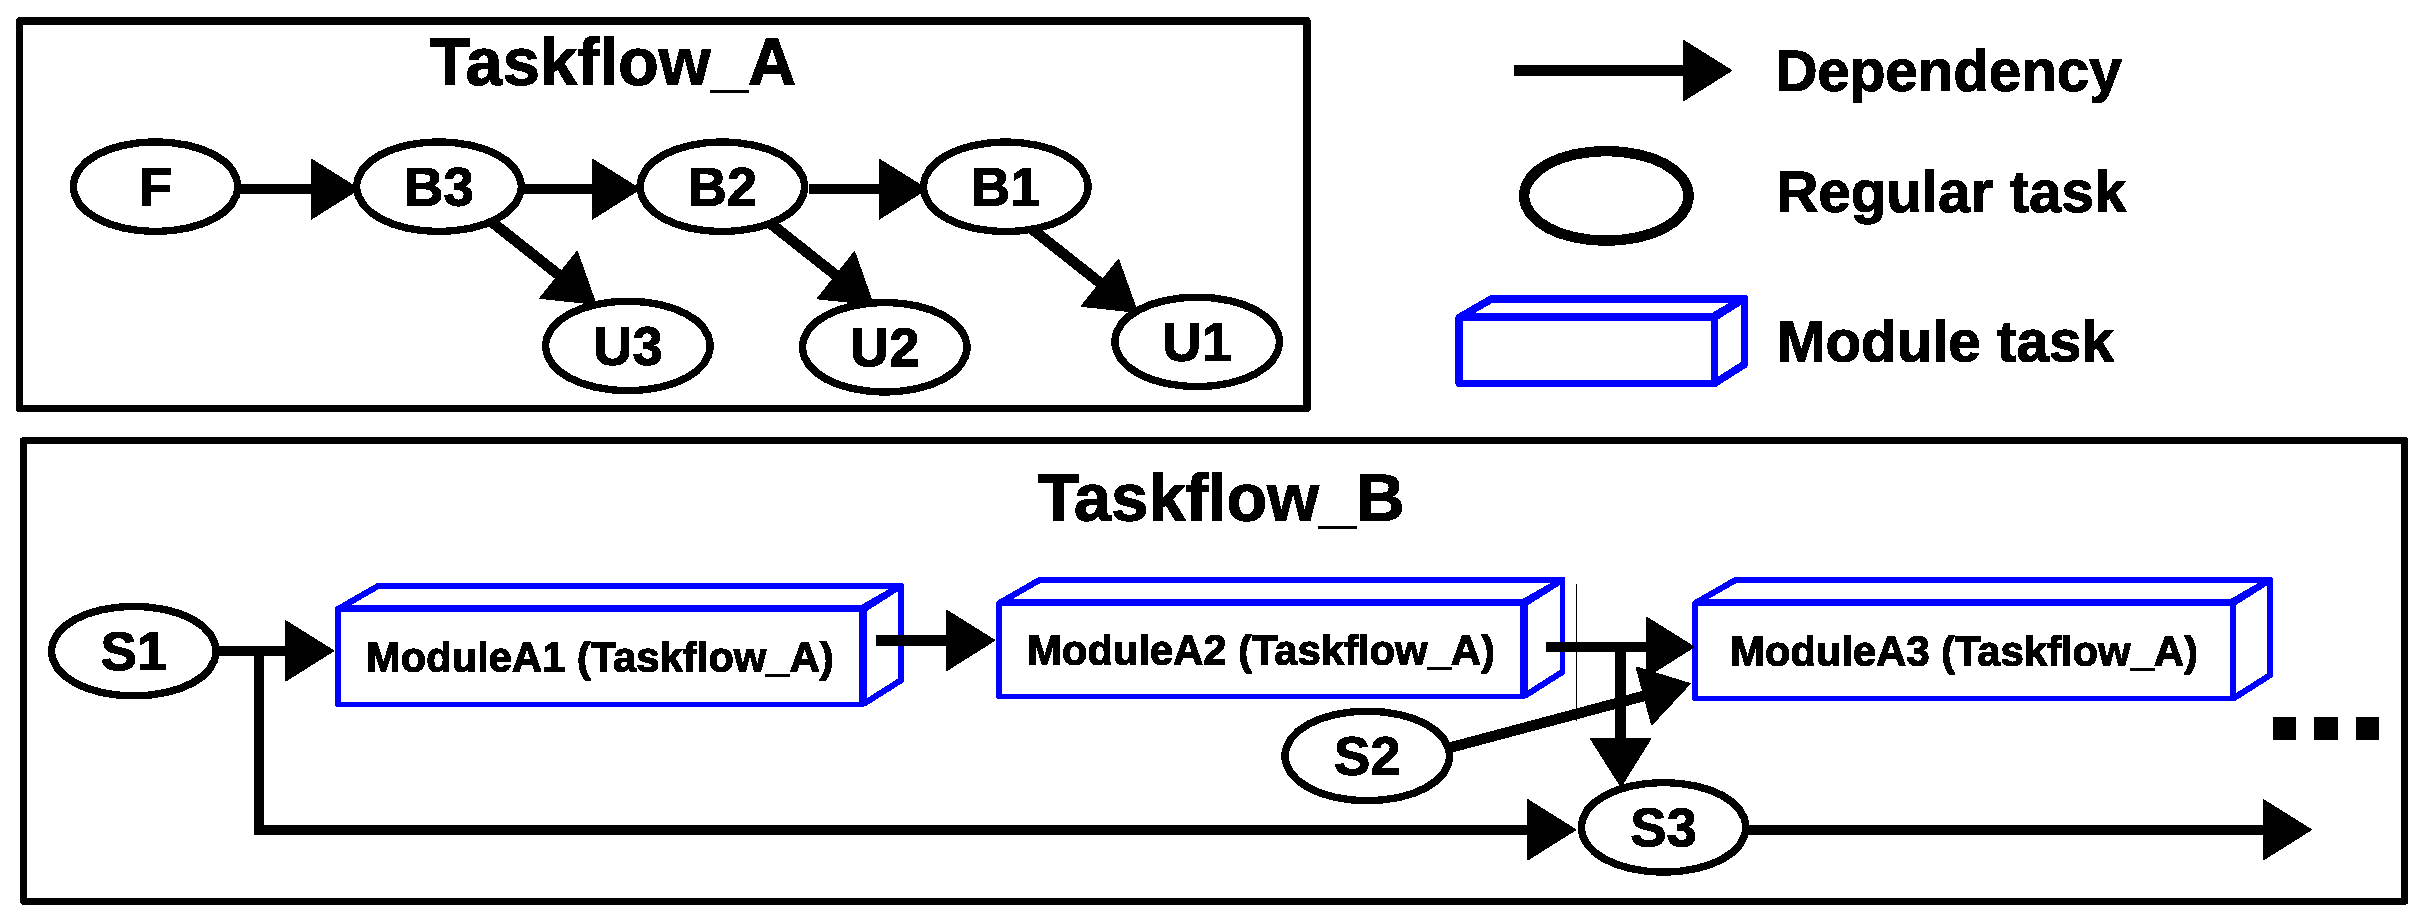
\includegraphics[width=.9\columnwidth]{Fig/first_example.eps}
  \caption{
    Using our composable task dependency graph to describe 
    a parallel neural network training workload.
    Taskflow object A represents one training iteration and is used to compose taskflow object B 
    for the entire training procedure.
  }
  \label{fig::taskflow_demo}
\end{figure}

In this paper, we introduce a powerful parallel programming model that enables efficient composition.
Our model is built on top of the modern C++ tasking library, 
Cpp-Taskflow~\cite{Huang_19_01},
but largely enhanced its capability with two key design changes:
(1) separating the task dependency graph and execution kernel
and (2) making the task dependency graph reusable and composable.
% through a new composable and reusable task 
% a new \textit{framework} interface.
In our model, a \emph{taskflow object} consists of a \textit{composable task dependency graph}
and user-friendly APIs to facilitate the creation of \textit{modular} and \textit{reusable}
parallel compute patterns and libraries.
These libraries can recursively compose large and complex parallel computations
on a single machine, taking advantage of multicore processing
while sharing thread resources to minimize overhead.
Figure \ref{fig::taskflow_demo} gives an example of 
using taskflow objects to describe a parallel training algorithm
of a deep neural network (DNN).
Taskflow object A represents a training pipeline.
Taskflow object B is composed of multiple As and other tasks to complete the training procedure.
Also, users can easily couple B with other parallel computations.
There is no redundancy from the programmability standpoint.
We summarize our contributions as follows:

\begin{itemize}[leftmargin=*]

\item \textbf{A new composable parallel programming model}. 
%We developed a composable task dependency graph 
We developed a composable task interface
to enable efficient composition of parallel workloads.
Our library lets users quickly describe a large parallel program 
through composition of modular and reusable task graphs that 
embed both regular and irregular compute patterns.
The program runs on a multicore machine with automatic scheduling optimization 
across different layers of composed tasks.


\item \textbf{A unified task composition interface}.
% We developed a unified framework interface that can capture a diverse set of tasks 
We developed a unified task graph construction interface that can capture a diverse set of tasks
from single sequential functions to large parallel dependent tasks or 
even out-of-context executions such as third-party calls and process forks.
The unified interface empowers developers with both explicit and implicit 
task graph composition to explore cross-layer optimizations
of their parallel workloads.

\item \textbf{A simple and efficient composition API}.
We developed a user-friendly API to describe task dependency graph composition using modern C++17 syntax.
Users can fully take advantage of the rich features of our engine
together with robust standard C++ libraries to productively compose many parallel applications.
Our library effectively separates users from 
low-level difficult concurrency details and offers \textit{transparent} scaling 
to many cores and future hardware generation.

\end{itemize}

Our work highlights the \textit{interface for composing parallel computing workloads}
as an important area to work in order to 
embrace high performance and high developer productivity at the same time.
Today's parallel workloads are large and complex, 
and are often combined with many sub-components of parallel computations
developed by different people.
Most existing parallel programming libraries feature domain-specific functions
to help users optimize their workloads but require them to fully 
understand the entire program structure.
This inevitably degrades the productivity of developers 
to collaborate on large projects through efficient composition.
Our library gives developers enough freedom to implement their own computations,
while supporting the performance optimizations across libraries.

\section{Composable Parallel Processing}

In this section, we discuss in detail our composable parallel task programming library
\textit{Cpp-Taskflow v2}\footnote{Source code is available in ~\cite{Cpp-Taskflow}}.
% 
% \epigraph{We aim to help software developers quickly write reusable, modular, and scalable parallel programs through composable task building blocks.}{--- \textup{Cpp-Taskflow v2's Project Mantra}}
 

\subsection{Cpp-Taskflow: A Modern C++ Parallel Task Programming Library}

We developed our composable task interface on top of Cpp-Taskflow,
an open-source parallel programming library based on task dependency graphs~\cite{Huang_19_01}. 
Cpp-Taskflow %has been used by many industrial and academic projects. It 
leverages the power of modern C++ and task-based approaches to enable
efficient implementations of parallel decomposition strategies.
Users focus on high-level description of dependent tasks for their parallel workloads,
leaving difficult details such as concurrency controls,
work stealing, and scheduling to the library.
Cpp-Taskflow supports both static and dynamic tasking in a uniform fashion. 
Static tasking lets users create task dependency graphs at programming time
while dynamic tasking occurs at runtime.
% These benefits allow Cpp-Taskflow to outperform existing task programming libraries
% such as OpenMP task and Intel Threading Building Blocks (TBB) FlowGraph~\cite{Huang_19_01, openmp, tbb}.
However, the ordinary task dependency graph in Cpp-Taskflow is not composable nor reusable.
Like other libraries, 
the lack of composability prevents users from modular design
to reuse available components of heavily refined task graphs.
Our goal is thus to enable a composable task interface
to enhance the capability of Cpp-Taskflow.


%\subsection{A New Framework Interface}
\subsection{A New Task Dependency Graph}

Cpp-Taskflow v2 introduces a new composable task interface, 
the \textit{\lstinline{tf::Taskflow} class}.
% the \textit{\lstinline{tf::Framework} class}.
%\lstinline{tf::Framework} is the main gateway to create a composable task dependency graph.
\lstinline{tf::Taskflow} is the main gateway to create a composable task dependency graph.
It inherits all the task construction methods from Cpp-Taskflow.
% Our design principle is to let users write simple and expressive composition code.
% By simple we mean the code explains itself.
%Listing \ref{task_creation} demonstrates how to create a framework of two static tasks A and B 
Listing \ref{task_creation} demonstrates how to create a task dependency graph with two tasks A and B 
where B runs after A and B spawns a new task B1 during runtime.
%A primary difference between a framework and the graph in Cpp-Taskflow is the separation of 
%A primary difference between Cpp-Taskflow v1 and v2 is the separation of 
% A primary change in Cpp-Taskflow v2 is the separation of the task dependency graph from executor. 
Cpp-Taskflow v2 separates the task dependency graph from executor.
% Users have full control over their framework graphs but are also responsible 
Users now have full control over their task dependency graphs but are also responsible 
for their lifetime.

\begin{lstlisting}[language=C++,label=task_creation,caption={Create a task dependency graph of two dependent static tasks and one dynamic task.}]
tf::Taskflow taskflow;

// Add a static task 
auto taskA = taskflow.emplace([](){
  std::cout << "Task A\n";
});

// Dynamic tasking
auto taskB = taskflow.emplace([](auto &subflow){
  std::cout << "Task B\n";
  subflow.emplace([](){
   std::cout << "Task B1\n";   
  });
});

taskA.precede(taskB);
\end{lstlisting}


\subsection{Execute a Task Dependency Graph}
A significant change by Cpp-Taskflow v2 is the decoupling of executor and task graph.  %the isolation of executor.   
Cpp-Taskflow v2 defines \lstinline{tf::Executor} class that has
a rich set of methods to run a task dependency graph.
%Cpp-Taskflow v2 defines \lstinline{tf::Executor} class to let users create an
%executor independent of task graphs.
%Cpp-Taskflow v2 defines a rich set of methods to run a task dependency graph.
%An executor has a rich set of methods to run a task dependency graph.
A task dependency graph can be run by an executor multiple times in arbitrary order.
Users can also give a predicate to specify the stopping criteria.
Listing \ref{taskflow_execution} demonstrates a set of common methods to run a task dependency graph.
Line 1:3 creates a taskflow object and adds some tasks.
Line 6 creates an executor.
An executor is nothing but a pluggable scheduler to dispatch tasks to threads in a shared pool.
The simplest way is to execute a task dependency graph only once via the
\lstinline{run} method (line 9).  
Alternatively, users can call \lstinline{run_n} to run a task dependency graph multiple times (line 13).
The bottommost call is \lstinline{run_until} (line 19),
which keeps running until the predicate becomes true.
All methods accept a callable object as a callback after the task execution completes.
To enable more asynchronous control,
each of these methods returns a \lstinline{std::future} for users 
to inspect the execution status or incorporate non-blocking program flow.
%
It should be noticed that running a task dependency graph multiple times exhibits 
the most basic composability, by which the same graph is encapsulated in a linear chain of tasks.

\begin{lstlisting}[language=C++,label=taskflow_execution,caption={Different ways to execute a task dependency graph.}]
tf::Taskflow taskflow;

// Add some tasks ...

// Create an executor with 4 threads
tf::Executor executor {4};

// Run the taskflow object once
auto fut = executor.run(taskflow); 
fut.get();

// Run the taskflow object 4 times with a callback
taskflow.run_n(taskflow, 4, [](){
  std::cout << "Finish!\n";
}).get();

// Run the taskflow object with a predicate 
int counter {4};
executor.run_until(taskflow, 
  [&](){ return --count == 0; }
).get();

\end{lstlisting}


\subsection{Task Dependency Graph Composition}

Task dependency graph composition is the most important feature in Cpp-Taskflow v2.
It allows users to create heavily optimized task dependency graphs and 
reuse them to compose larger graphs and so on so forth.
The \lstinline{tf::Taskflow} class defines a method \lstinline{composed_of} to enable composition.
Specifically, the caller taskflow object adds a module task of the callee taskflow object. 
Listing~\ref{taskflow_composition} shows an example of taskflow object composition.
% and Figure~\ref{fig::taskflow_composition} shows the composed graph.
Line 1:10 creates a taskflow object with three dependent tasks A1, A2, and A3. 
% where A3 runs after A1 and A2.
Line 12:19 creates another taskflow object with three tasks B1, B2, and B3.
Line 22 adds a module task from the first taskflow object and
line 25:27 specifies the dependency between tasks.
Unlike the \lstinline{emplace} method that creates a \textit{regular task}, 
the \lstinline{composed_of} method creates a \textit{module task} in the graph.
A module task is a special task that is aware of which taskflow object to probe
during its execution context.
%
We would like to highlight three points of our composition interface.
First, there is no copy during the composition, 
leading to efficient graph sharing and resource utilization.
We have strived to resolve many scheduling conflicts due to shared tasks,
while providing a high-level execution API to completely separate this low-level controls 
from users.
Second, recursive and nested composition are feasible.
A taskflow object can be used to compose multiple taskflow objects and the resulting taskflow object
can compose another taskflow object with no restriction.
During the composition, user can add free-standing tasks to the graph
to perform computation across different task layers.
Adding dependency is extremely easy and flexible through the \lstinline{precede} method.
Finally, the module task works seamlessly with both static and dynamic tasking.
This gives users a powerful and unified tasking interface to accomplish 
large and complex parallel workloads.

%\begin{lstlisting}[language=C++,label=taskflow_composition,caption={Cpp-Taskflow v2 task object composition code for Figure \ref{fig::taskflow_composition} (19 LOC and 167 tokens).}]
\begin{lstlisting}[language=C++,label=taskflow_composition,caption={Cpp-Taskflow v2 taskflow object composition code (19 LOC and 167 tokens).}]
tf::Taskflow fA;

// Add three tasks
auto [A1, A2, A3] = fA.emplace(
 [](){ std::cout << "Task A1\n"; },
 [](){ std::cout << "Task A2\n"; },
 [](){ std::cout << "Task A3\n"; }
);

A3.gather(A1, A2);

tf::Taskflow fB;

// Add three tasks
auto [B1, B2, B3] = fB.emplace(
 [](){ std::cout << "Task B1\n"; },
 [](){ std::cout << "Task B2\n"; },
 [](){ std::cout << "Task B3\n"; }
);

// Compose taskflow object
auto moduleA = fB.composed_of(fA);

// Build dependency between module and regular tasks
B1.precede(moduleA);
B2.precede(moduleA);
moduleA.precede(B3);

\end{lstlisting}

%\begin{figure}[!h]
%  \centering
%  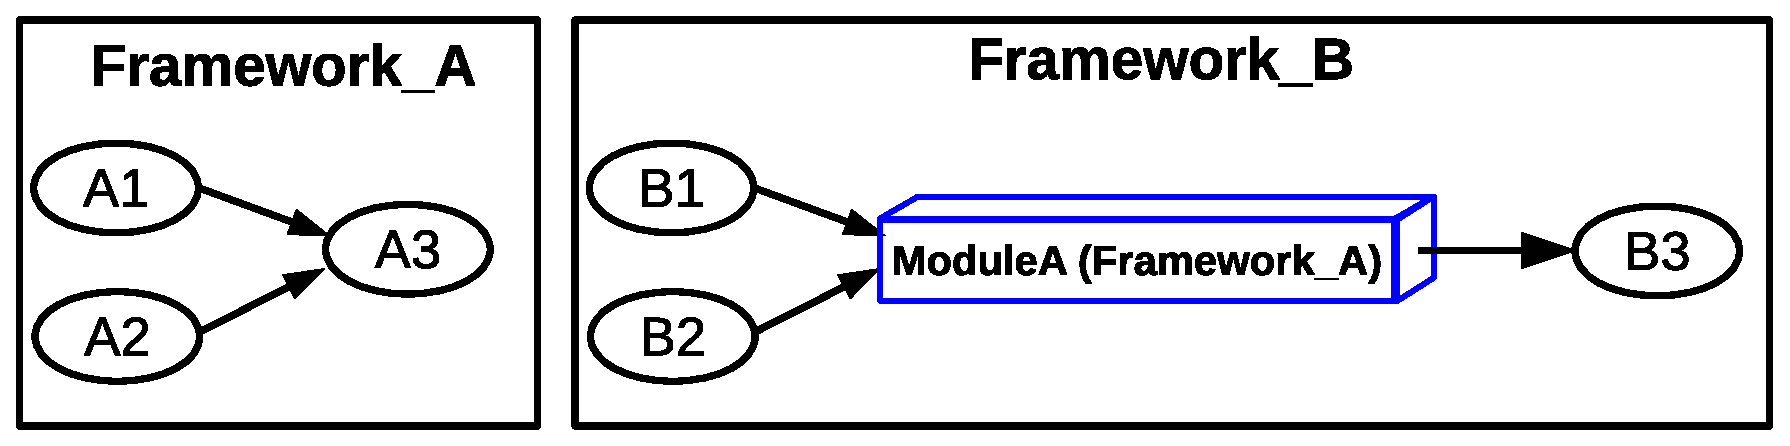
\includegraphics[width=.9\columnwidth]{Fig/composition.eps}
%  \caption{
%    Taskflow object A consists of three dependent tasks.
%    Taskflow object B consists of three dependent tasks and a module task composed of taskflow object A.
%  }
%  \label{fig::taskflow_composition}
%\end{figure}

At this point, we are interested in the difference between our composition code
and existing libraries.
%and the counterparts using existing libraries.
% Listing~\ref{omp_composition} and 
Listing~\ref{tbb_composition} is the 
implementations of Listing~\ref{taskflow_composition} using TBB flow graph~\cite{tbb}. 
%implementations of Figure~\ref{fig::taskflow_composition} using TBB FlowGraph. 
%both libraries do not have a clear composition interface and the best way 
%to emulate our example is handwritten function calls.
%
%
As shown in the two listings,
Cpp-Taskflow v2 has the least lines of code % and tokens 
and is more readable compared with TBB code.   
%Due to the lack of graph concept, 
% When creating a modular system, instead of creating a monolithic application (where the smallest component is the whole), 
% modularization is hard to realized in OpenMP 
% tasks are belonging to the same in OpenMP  
%tasks are under the same scope in OpenMP
%and we encapsulate tasks in individual functions to emulate composition. 
% OpenMP has no concept of task graph, so we encapsulate tasks in 
% individual functions to emulate composition. 
% Due to the lack of task graph concept,  is not applicable 
% it's hard to abstract the parallel 
% employ module design using OpenMP.
% it's hard to abstract a parallel pattern as a module in OpenMP.
% apply OpenMP to 
% hierarchical design
% Due to the lack of task graph, OpenMP has only 
% The lack of task graph makes OpenMP 
% For TBB, 
To our best knowledge, TBB has no API to directly compose task graphs, so we have to 
capture the task graph into another task and execute the task graph. This results in 
longer lines of code and tends to produce bugs if one forgets to execute the task graph.
This example clearly shows the conciseness and ease-of-use of the task 
composition interface in Cpp-Taskflow v2.  

% Fairly speaking, the OpenMP implementation is not  
% OpenMP has no concept of task graph and 

%\begin{lstlisting}[language=C++,label=omp_composition,caption={OpenMP hard-coded composition code of Figure~\ref{fig::framework_composition} (46 LOC and 175 tokens).}]
%void task_set_A() {
%  int a1, a2;
%  #pragma omp parallel 
%  {
%    #pragma omp single 
%    {
%      #pragma omp task depend (out: a1) 
%      {
%        std::cout << "Task A1\n";
%      }
%      #pragma omp task depend (out: a2) 
%      {
%        std::cout << "Task A2\n";
%      }
%      #pragma omp task depend (in: a1, a2)
%      {
%        std::cout << "Task A3\n";
%      }
%    }
%  } 
%}
%
%void task_set_B() {
%  int b1, b2, a;
%  #pragma omp parallel 
%  {
%    #pragma omp single 
%    {
%      #pragma omp task depend (out: b1) 
%      {
%        std::cout << "Task B1\n";
%      }
%      #pragma omp task depend (out: b2) 
%      {
%        std::cout << "Task B2\n";
%      }
%      #pragma omp task depend (in: b1, b2) 
%                       depend (out: a)
%      {
%        task_set_A();
%      }
%      #pragma omp task depend (in: a)
%      {
%        std::cout << "Task B3\n";
%      }
%    }
%  }
%}
%\end{lstlisting}


%\begin{lstlisting}[language=C++,label=tbb_composition,caption={TBB hard-coded composition code of Figure~\ref{fig::taskflow_composition} (48 LOC and 256 tokens).}] 
\begin{lstlisting}[language=C++,label=tbb_composition,caption={TBB hard-coded composition code (48 LOC and 256 tokens).}] 
using namespace tbb;
using namespace tbb::flow;

graph fA;

continue_node<continue_msg> A1(fA, [] 
  (const continue_msg&) {
    std::cout << "Task A1\n"; 
  }
);
continue_node<continue_msg> A2(fA, [] 
  (const continue_msg&) {
    std::cout << "Task A2\n"; 
  }
);
continue_node<continue_msg> A3(fA, [] 
  (const continue_msg&) {
    std::cout << "Task A3\n"; 
  }
);

make_edge(A1, A3);
make_edge(A2, A3);

graph fB;

continue_node<continue_msg> B1(fB, [] 
  (const continue_msg&) {
    std::cout << "Task B1\n"; 
  }
);
continue_node<continue_msg> B2(fB, [] 
  (const continue_msg&) {
    std::cout << "Task B2\n"; 
  }
);
continue_node<continue_msg> B3(fB, [] 
  (const continue_msg&) {
    std::cout << "Task B3\n"; 
  }
);
continue_node<continue_msg> moduleA(fB, [&] 
  (const continue_msg&) {
    A1.try_put(continue_msg());
    A2.try_put(continue_msg());
    fA.wait_for_all();
  }
);

make_edge(B1, moduleA);
make_edge(B2, moduleA);
make_edge(moduleA, B3);

\end{lstlisting}

In addition to the composability, another useful feature %of framework interface is the
is the modularity.  Through \emph{inheritance} from \lstinline{tf::Taskflow} class, users
can define their own task dependency graph class as a \emph{single module}.  
The task dependency graph composition and execution APIs can be directly applied to
the customized class as well, obviating the need of an additional wrapper.

% \begin{lstlisting}[language=C++,label=customization,caption={Customize task dependency graph through class inheritance.}] 
% class UserGraph: public tf::Taskflow {
%   public:
% };
% %\end{lstlisting}
% Due to C++'s object
% slicing the composition and execution APIs can be directly applied to
% the customized class as well, obviating the need of an additional wrapper.
%Listing~\ref{framework_module} demonstrates a customized framework class.

%\begin{lstlisting}[language=C++,label=framework_module,caption={Customize task dependency graph through class inheritance.}] 
%enum class Operator { plus, multiply };
%
%// Define a parallel reduce task graph 
%struct ReduceFramework: public tf::Framework {
%  ReduceFramework(std::vector<int>& data, 
%    Operator op) {
%    if(op == Operator::plus) {
%      result = 0;
%      reduce(data.begin(), data.end(), 
%             result, std::plus<int>());
%    }
%    else {
%      result = 1;
%      reduce(data.begin(), data.end(), 
%             result, std::multiplies<int>());
%    }
%  }
%  int result;
%};
%
%std::vector<int> data;
%
%ReduceFramework f1(data, Operator::plus);
%ReduceFramework f2(data, Operator::multiply);
%
%// Declare executor
%tf::Taskflow taskflow; 
%
%// Run the custom frameworks
%taskflow.run(f1).get();
%taskflow.run(f2).get();
%
%std::cout << f1.result << std::endl;  
%std::cout << f2.result << std::endl;  
%
%\end{lstlisting}


With the composability and modularity, a complex design
can be decomposed into small components with different parallel patterns. Users
can implement and test those patterns individually and combine them
in various ways such as nested or concatenation to deliver complex functionality. 
This can substantially increase programmers' productivity as it enables a
structural and efficient way for software engineering.  

% Cpp-Taskflow v2 allows composition of tasking graphs to build .
% Similar to the task insertion, a tasking graph composes other tasking graphs
% via the \lstinline{composed_of} method. 

\subsection{Unified Task Execution}
% Cpp-Taskflow v2  
% enhances the 
% redesigns the execution kernel by unifying the 
% seamless
% To enable seamless integration of framework with existing task types in
% Cpp-Taskflow, Cpp-Taskflow v2 adds two changes to the execution
% kernel to enable the reusability and composability of framework. 

%To enable seamless integration of the new task dependency graph with existing task types in
%Cpp-Taskflow, Cpp-Taskflow v2 modifies the execution
% kernel to enable the reusability and composability of framework. 
%kernel to enable the reusability and composability of framework. 

Cpp-Taskflow v2 modifies the execution kernel
to enable seamless integration of the reusable and composable task dependency graph with existing task types.
To make a task dependency graph reusable, it's necessary to ensure the
graph remains unchanged after each execution.  
During runtime, a task might expand the graph by spawning
new nodes to precede the parent node such as dynamic tasking.
% Static tasking does
% not affect the structure of task dependency graph while dynamic tasking might
% expand the graph by spawning new nodes to precede the parent node during
% runtime.  
As a result, in Cpp-Taskflow v2 a task that spawns new tasks will restore its own
precedence before scheduling its successor tasks.  
Letting each task perform the restoration on itself also minimizes the overhead. 

Apart from the regular tasks, a task dependency graph can have module tasks through
composing other graphs.  The execution flow of module task is similar 
to dynamic tasking except that a module task directly dispatches the composed graph rather 
than a subflow.
%The execution flow of a module task is similar to the dynamic tasking where the node will be visited twice:
A module task will be executed twice: 
\begin{itemize}[leftmargin=*]
  \item First time:
    \begin{itemize}
      \item The executor first collects the source and sink tasks in the composed graph and  
        let the sink tasks precede the module task.
      \item The executor dispatches the source tasks to execution. 
    \end{itemize}
  \item Second time:
    \begin{itemize}
      \item The executor clears the successor of sink tasks in composed graph. 
      \item The executor dispatches the module task's successors to execution.
    \end{itemize}
\end{itemize}
Figure~\ref{fig::scheduling} is an example that illustrates scheduling a module task.
% As a module node has spawn new tasks, a module node also needs to restore its own
% precedence before scheduling its successor tasks.
% During task execution, we use the pointer to the composed framework to
% separate the execution flow of  module tasks from regular tasks.
% Listing~\ref{executor_pseudocode} is the pseudo code of Cpp-Taskflow v2's
% execution kernel.  Line 1-19, 20-23 and 24-38 are the execution flows for
% module task, static tasking and dynamic tasking respectively.  Tasks that have
% spawn new tasks restores its dependency at line 41-43.  A task dispatches its
% successor tasks at line 46.
% 
% \begin{lstlisting}[language=C++,label=executor_pseudocode,caption={The pseudo code of the task execution kernel.}]  
% if(task.module_pointer) {
%   // Module task 
%   auto first_time = task.is_spawned();
%   if(first_time) {
%     // Collect the source tasks
%     srcs = source_task(task.module_pointer);
%     // Set the successor of sink tasks 
%     sinks = sink_task(task.module_pointer);
%     sinks.precede(task);
%     // Dispatch the composed framework 
%     dispatch(srcs);
%     task.set_spawned();
%     return ;
%   }
%   else {
%     // Second time 
%     clear_successor(task.module_pointer);
%   }
% }
% else if(task.static_tasking()) {
%   // Static tasking
%   invoke(task.work);
% }
% else {
%   // Dynamic tasking  
%   auto first_time = task.is_spawned();
% 
%   SubflowBuilder subflow;
%   invoke(task.work, subflow); 
% 
%   if(first_time) {
%     task.set_spawned();
%     dispatch(subflow);
%     if(!subflow.detached()) {
%       return ;
%     }
%   }
% }
% 
% // Only module task & dynamic tasking 
% if(!task.static_tasking() or task.module_pointer) {
%   task.restore_dependency();
% }
% 
% // Dispatch successor tasks
% dispatch(task.successors);
% 
% \end{lstlisting}


% During runtime a module task dispatches the
% composed task dependency graph and makes the sink nodes precede it. 


\begin{figure}[!h]
  \centering
  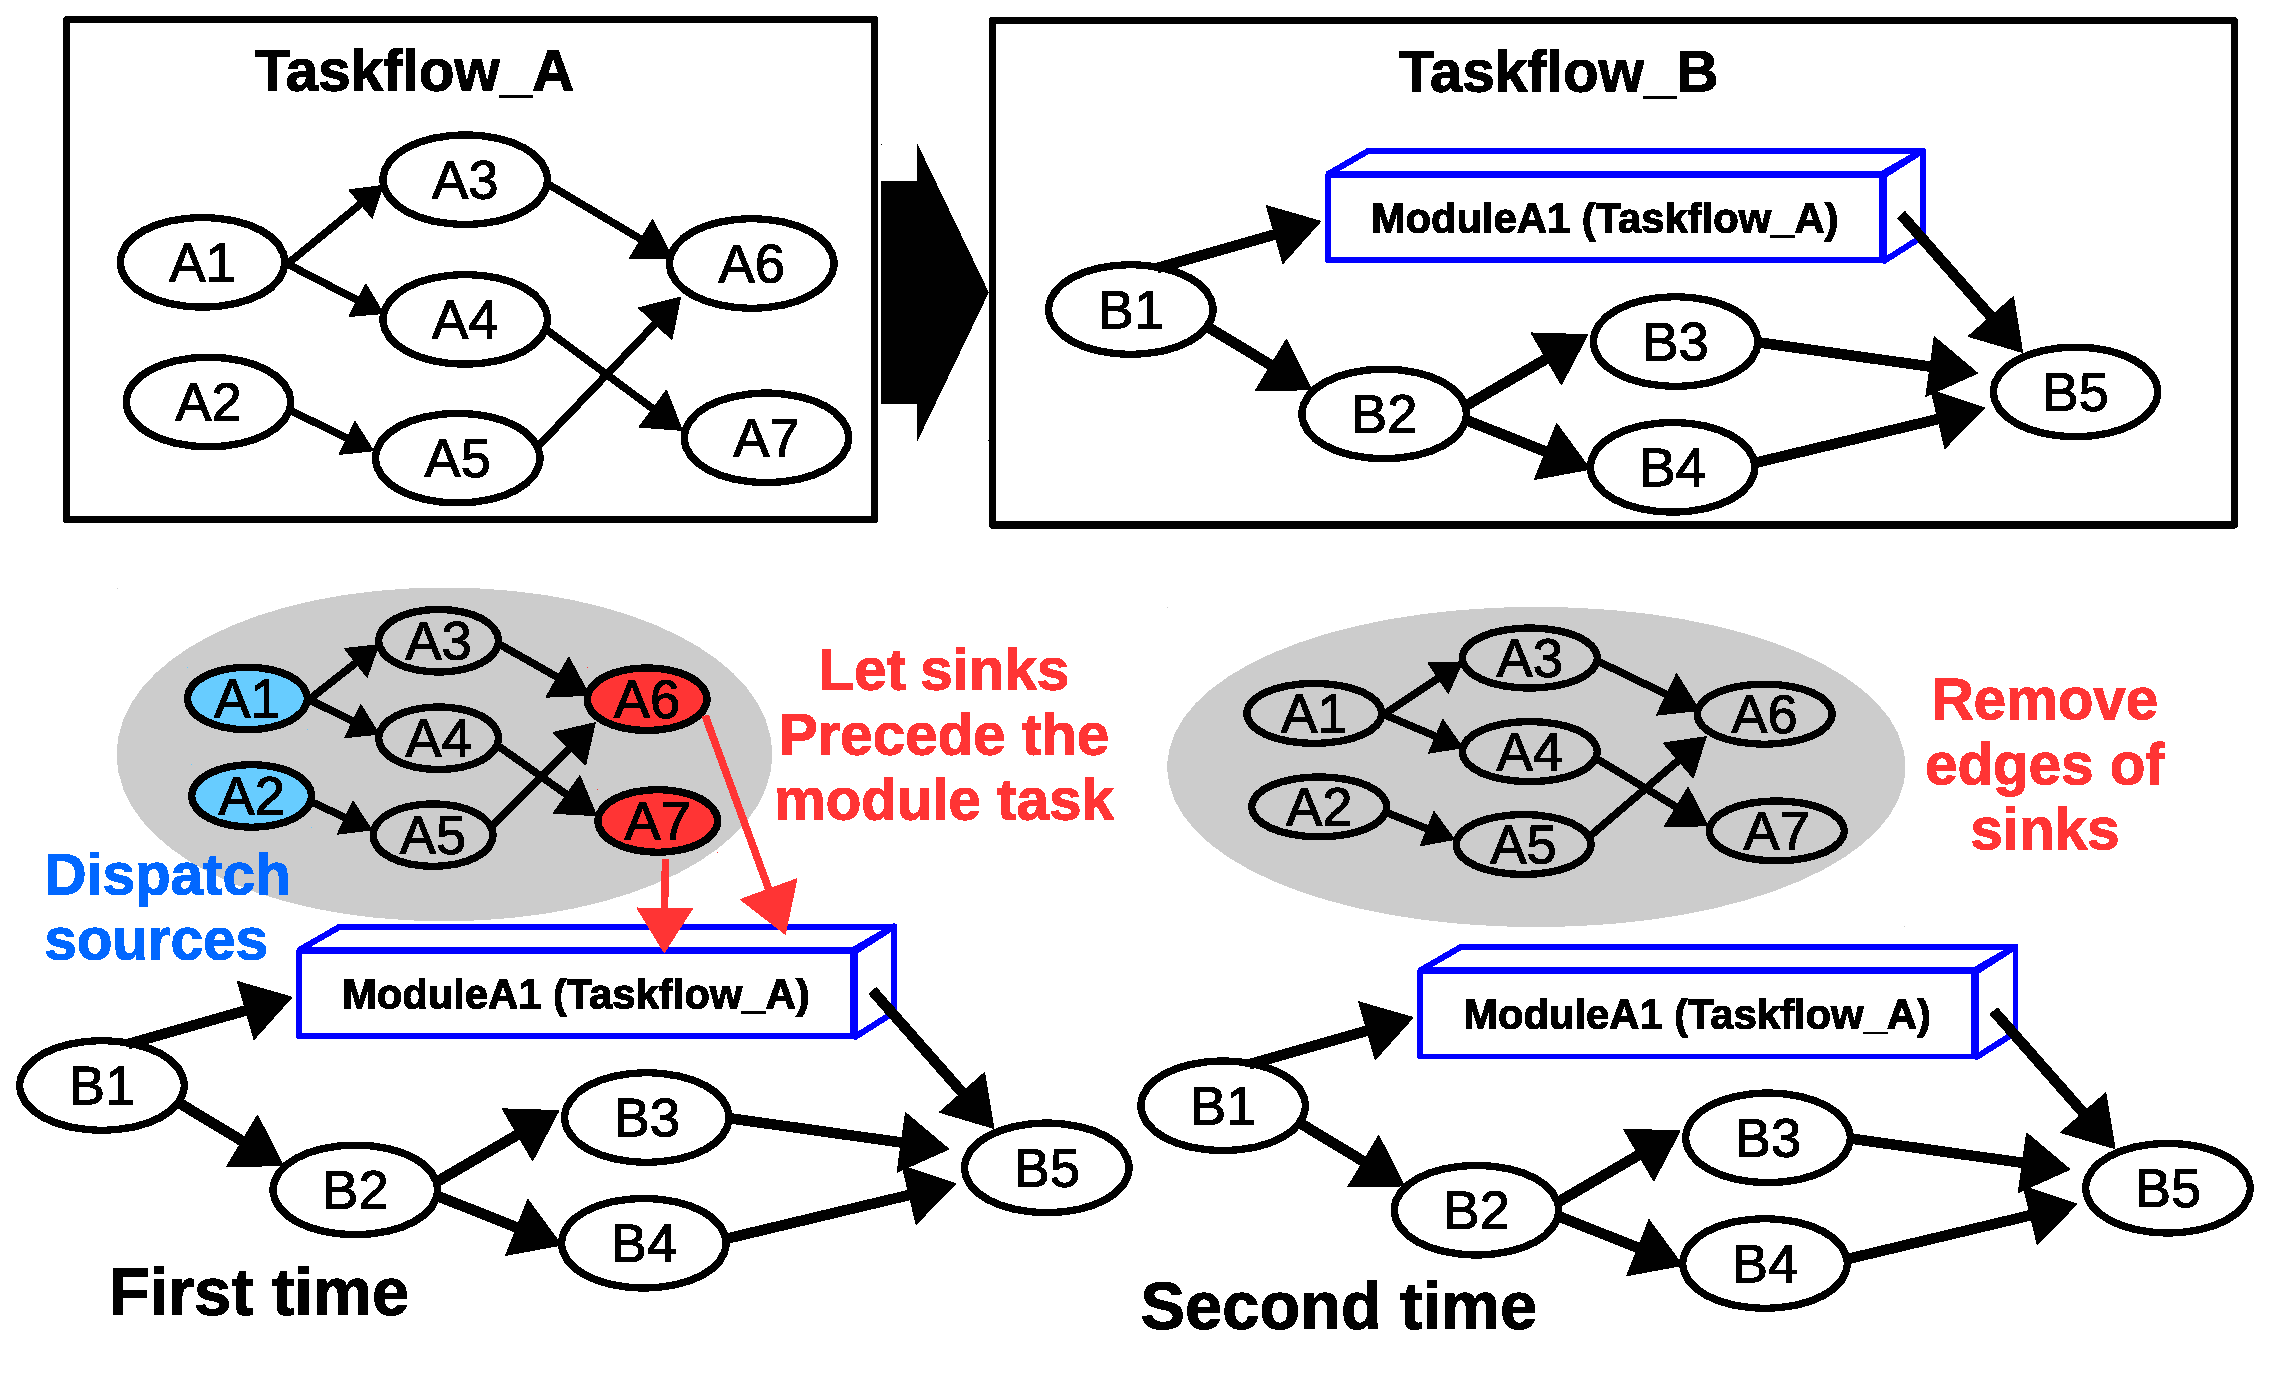
\includegraphics[width=.95\columnwidth]{Fig/scheduling.eps}
  \caption{
     %The task dependency graph of the wavefront computing pattern.
    An example to illustrate the execution of module task.
   }
  \label{fig::scheduling}
\end{figure}



\subsection{Visualize a task dependency graph with both regular and module tasks.}
% Visualization is a useful technique to assist developers in program debugging,
% and for parallel programming the ability to visually inspect the execution flow
% would be extremely helpful.
% and this has been supported in the \lstinline{tf::Framework} class.  
Cpp-Taskflow v2 provides the same APIs as Cpp-Taskflow to support visualization
of task dependency graph to facilitate debugging.
%so developers can see the task execution flow. 
A taskflow object can be assigned a name by the \lstinline{name} method and it
has a \lstinline{dump} method to export its task dependency graph in DOT language~\cite{dot}.
A module task is represented by a \emph{cuboid} to differentiate from the regular tasks.
Figure~\ref{fig::framework_dump} shows an example of visualizing composed task dependency graphs.
% To differentiate module task from the regular ones, a module 
% A framework object can be assigned a name by the \lstinline{name} method and it
% has a \lstinline{dump} method to export its task dependency graph in DOT language~\cite{dot}.
% Listing~\ref{visualization} shows how to set the name and visualize the task dependency
% graph of a framework object and Figure~\ref{fig::framework_dump} is a DOT graph
% exported from a framework.  When visualizing a framework, we not only dump
% the framework itself but also all the composed frameworks so that users can 
% have a comprehensive view of the execution flow.
% \begin{lstlisting}[language=C++,label=visualization,caption={Visualization of composable task dependency graphs.}]
% tf::Taskflow taskflow;
% 
% // Set the graph's name
% taskflow.name("Example");
% 
% // Add some tasks ...
% 
% // Dump the task dependency graph of the framework
% std::cout << framework.dump() << std::endl;
% 
% \end{lstlisting}


\begin{figure}[!h]
  \centering
  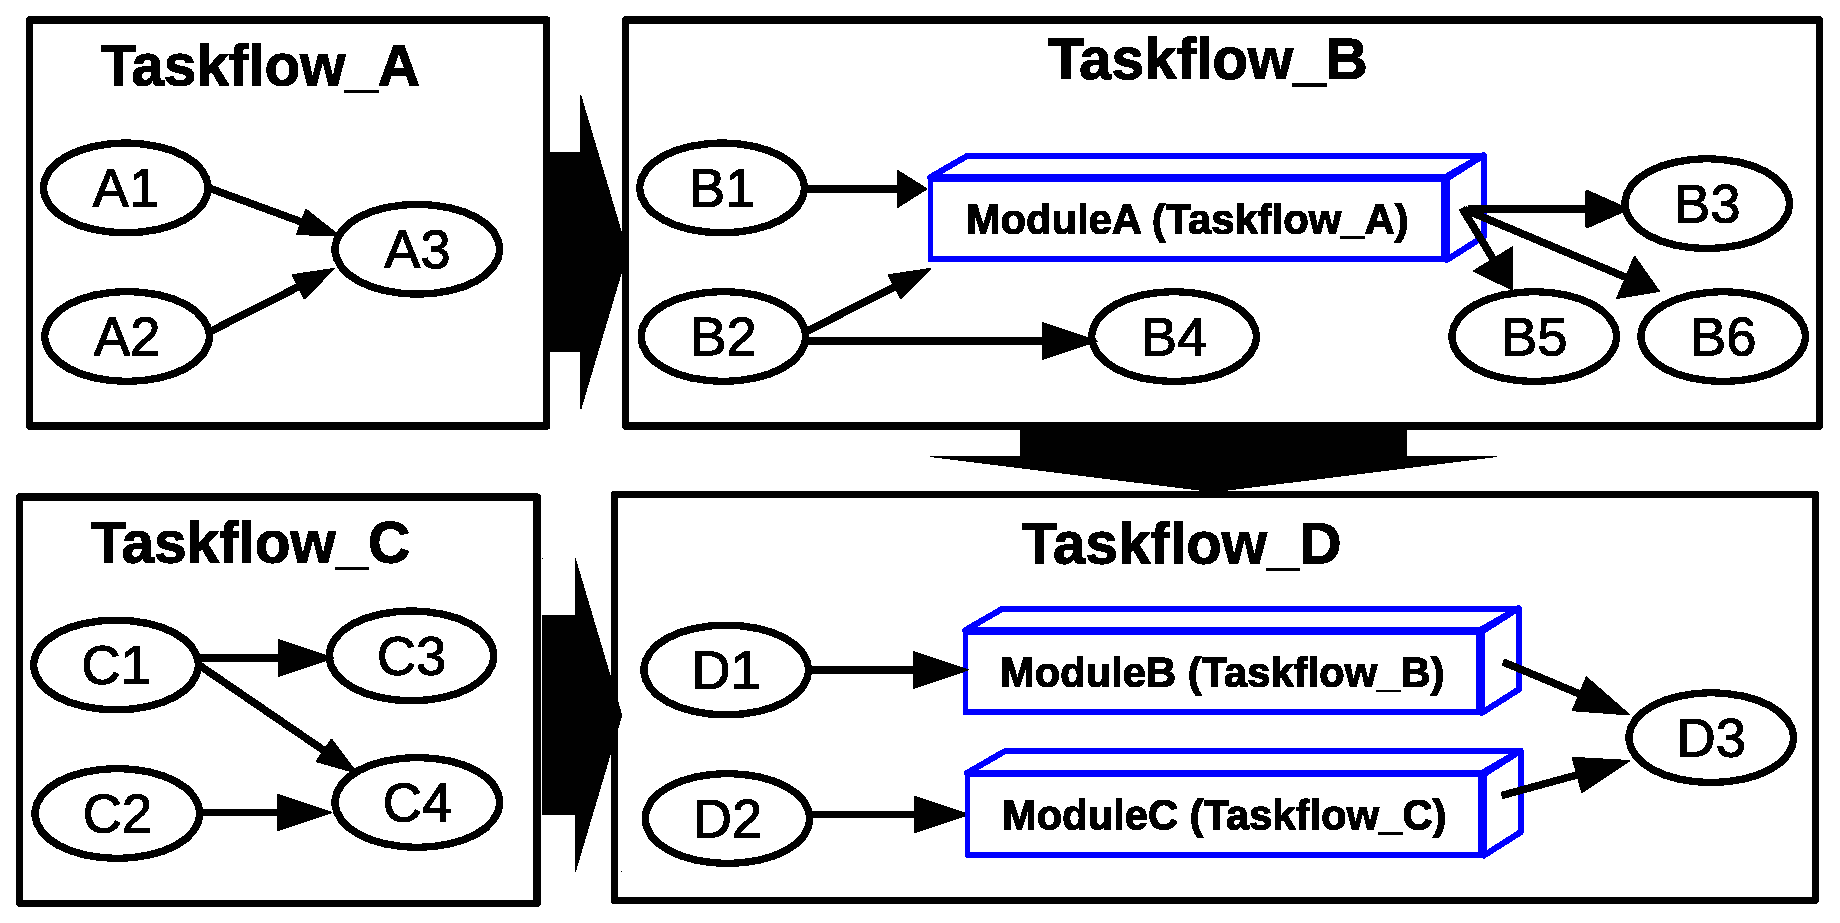
\includegraphics[width=.9\columnwidth]{Fig/visualization.eps}
  \caption{
     Visualize the task dependency graph D with its regular and module tasks. 
     Note the arrows between taskflow objects are added deliberately here for clarity.
   }
  \label{fig::framework_dump}
\end{figure}


\section{Evaluation}
We conduct experiments to emulate two real-world applications, 
a parallel machine learning hyperparameter
search and a 
Very-large-scale integration (VLSI) circuit timing analysis. 
% We conduct experiments using two types of benchmarks to evaluate Cpp-Taskflow v2, 
% micro-benchmarks and real-world applications. 
% The micro-benchmarks are to measure:
% task scheduling overhead of frameworks with regular and irregular task graph structures 
% and the runtime of a composed framework. 
% and the runtime of repeatedly executing a framework. 
% Note that executing a framework multiple times is similar to executing a linearized framework,
% by which all tasks encapsulate the same graph. So this experiment can also be 
% regarded as a way to profile the execution of a composed task graph.
% Those applications contain complex dependency which is suitable to be handled using the task dependency graph model. 
We focus on comparison with TBB as both Cpp-Taskflow v2 and TBB 
adopt task dependency graph for programming model. 
We demonstrate Cpp-Taskflow v2 achieves comparable performance with less software development effort using 
the task graph composition.

%In this experiment 
% We demonstrate how to use graph composition to 
% quickly build complex applications and the composability 
% can effectively reduce the software development effort.

The experiment platform has 128 GB memory and a 2.5 GHz Intel Xeon W-2175 processor with 14 physical cores 
and 28 threads. The operating system is Ubuntu 18.04.2. We use the library provided APIs to
control the number of threads and the system utility \lstinline{taskset}
to pin each thread to a specific core to minimize the migration overhead.  
All programs are compiled using g++-7.4 with optimization flag \lstinline{O2} and
C++ standard flag \lstinline{-std=c++17}. 
%We use OpenMP version 4.5 and Intel
We use Intel TBB 2019 Update 2 (flow graph) as the baseline for evaluation. 


%\subsection{Machine Learning Hyperparameter Search}
\subsection{Machine Learning Application}
% In this section, we introduce a parallel hyperparameter search approach for 
% deep neural network (DNN) on the MNIST dataset~\cite{mnist}.
% and we will 
% highlight the benefits of composability in building a complex application.
% with especially focus on the benefits , the benefits of using composable framework 
% using the composable task dependency graph to build a complex application.
% focus on the benefits brought by the reusability and composability of 
% tasking graph. 
Machine learning involves lots of computations and parallel computing plays a key role 
in building machine learning applications.
Deep neural network (DNN) is a fundamental machine learning model and a DNN
typically has many parameters to tune such as learning
rate, layer number, and weight initialization~\cite{Hyperparameter_2013}. 
Finding a good parameter set is an important topic
in machine learning study and many approaches have been 
proposed~\cite{Hyperparameter_2013}~\cite{random_search}~\cite{bayesian_search}~\cite{grid_search}.
% The combination of those parameters will have a significant impact on the model's
% effectiveness.  Therefore, finding a good parameter set is an important topic
% in machine learning study and many approaches have been 
% proposed~\cite{Hyperparameter_2013}~\cite{random_search}~\cite{bayesian_search}.
% A critical concern of hyperparameter search is the efficiency, as the
% search can be very time-consuming due to the laborious training procedure and
% the combinatorial explosion in search space. 
%The architectures of different machine learning models can vary greatly and 
%their task graphs can be very distinct. For example, a convolutional
%neural network v.s. a recurrent neural network. 
%Therefore, hardcoding those machine learning models in a monolithic 
%task graph can be very challenging and error-prone. 
%With Cpp-Taskflow v2, we can create 
%% With the framework interface of Cpp-Taskflow v2, 
An intuitive way to explore the parameter space is to concurrently train
multiple DNNs with different parameter sets. 
%This approach is to increase the throughput via concurrency.
%The key idea here is to increase the throughput via concurrency.
We emulate this process by creating a parallel DNN training framework on the MNIST dataset~\cite{mnist}. 
In this framework, we train multiple DNNs concurrently and synchronize them 
every epoch and shuffle the data for next epoch.
% to perform data shuffle. 
% We design a parallel hyperparameter search approach to speed up the parameter set
% exploration by training multiple DNNs concurrently with different learning rates.
% The key idea is the same as the grid-search approach~\cite{grid_search}, where
% each DNN is independently trained to each other so that the concurrency can increase the
% throughput. 
% Figure~\ref{fig::dnn_overview} is the overview of the framework.
% Each DNN is trained with a different learning rate for one epoch and 
%we synchronize all DNN after one epoch training and examine the accuracy of each DNN. 

% We segment the backward propagation into 
% a gradient calculation and a weight update task and 
%\begin{figure}[!h]
%  \centering
%  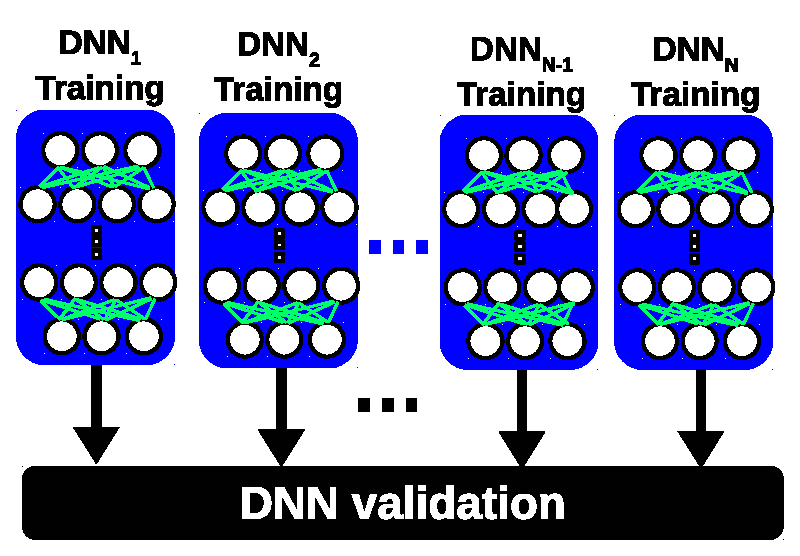
\includegraphics[width=.8\columnwidth]{Fig/ParallelDNN.eps}
%  \caption {
%    An overview of parallel hyperparameter search approach. We train multiple DNNs concurrently 
%    with each DNN takes a different learning rate.
%  }
%  \label{fig::dnn_overview}
%\end{figure}

% With Cpp-Taskflow v2's task graph composition, we first create a task graph 
% for a batch training. Then we compose the task graph to create a  
% task graph for a single epoch. 
% To implement this framework, we need to construct a task graph for training all DNNs.  
% An intuitive implementation is to hard-code all DNNs in a monolithic task graph, 
% but this method has two issues. 
% First, this method might lead to memory exhaustion as it flattens all DNN task graphs. 
% Second, the flattened task graph is hard to debug as it mixes both the inter- and intra-connections 
% of all task graphs.
% The hardcoding method can consume too much memory 
% is very challenging and error-prone. 
% With Cpp-Taskflow v2's task graph composition, we can instantiate a task graph
% for each DNN from a DNN training framework and compose them into a parallel
% hyperparameter search framework.
% This is more efficient and scalable compared with the hardcoding method. 
% and compose the 
%This can be solved by Cpp-Taskflow v2's task graph composition. we can create a DNN training framework 
% to enable parallelism within training procedure. 
%Since all DNNs have the same structure , we make a modular interface for the DNN's task dependency graph 
%and instantiate as many modules as the DNNs from the interface.
%For Cpp-Taskflow v2, this can be easily realized through the framework interface.
%For Cpp-Taskflow v2, this can be easily realized using framework's composability. 
%The idea is to compose frameworks  hierarchically 
% To implement the proposed framework, we first adopt the task pipelining
% strategy proposed by~\cite{Cpp-Taskflow} to build the task dependency graph for DNN training.
To implement the proposed framework with Cpp-Taskflow v2, we first create a \lstinline{TrainingPattern} class that performs 
a training pass (forward/backward propagation) over a batch of data. 
We use the task pipelining strategy proposed by~\cite{Huang_19_01} in the \lstinline{TrainingPattern} 
to enable parallelism.
Then, we build a \lstinline{TrainingEpoch} class to iterate through all batches
by composing each \lstinline{TrainingPattern} into a linearized task graph. 
Lastly, we gather those \lstinline{TrainingPatterns} with a data shuffle task
into a \lstinline{ParallelDNNTraining} task graph. Figure~\ref{fig::dnn_composition} 
depicts the framework. 
For TBB, we first use the flow graph interface to build the \lstinline{TrainingPattern} for each DNN. 
Then we create another flow graph for \lstinline{ParallelDNNTraining}.
The \lstinline{ParallelDNNTraining} flow graph explicitly captures a \lstinline{TrainingPattern} in a node 
and launches the training during execution. 
% TBB flow graph does not offer graph composition APIs and we work around this by
% explicitly capturing task graphs into other graphs' tasks and manually launching the execution.

\begin{figure}[!h]
  \centering
  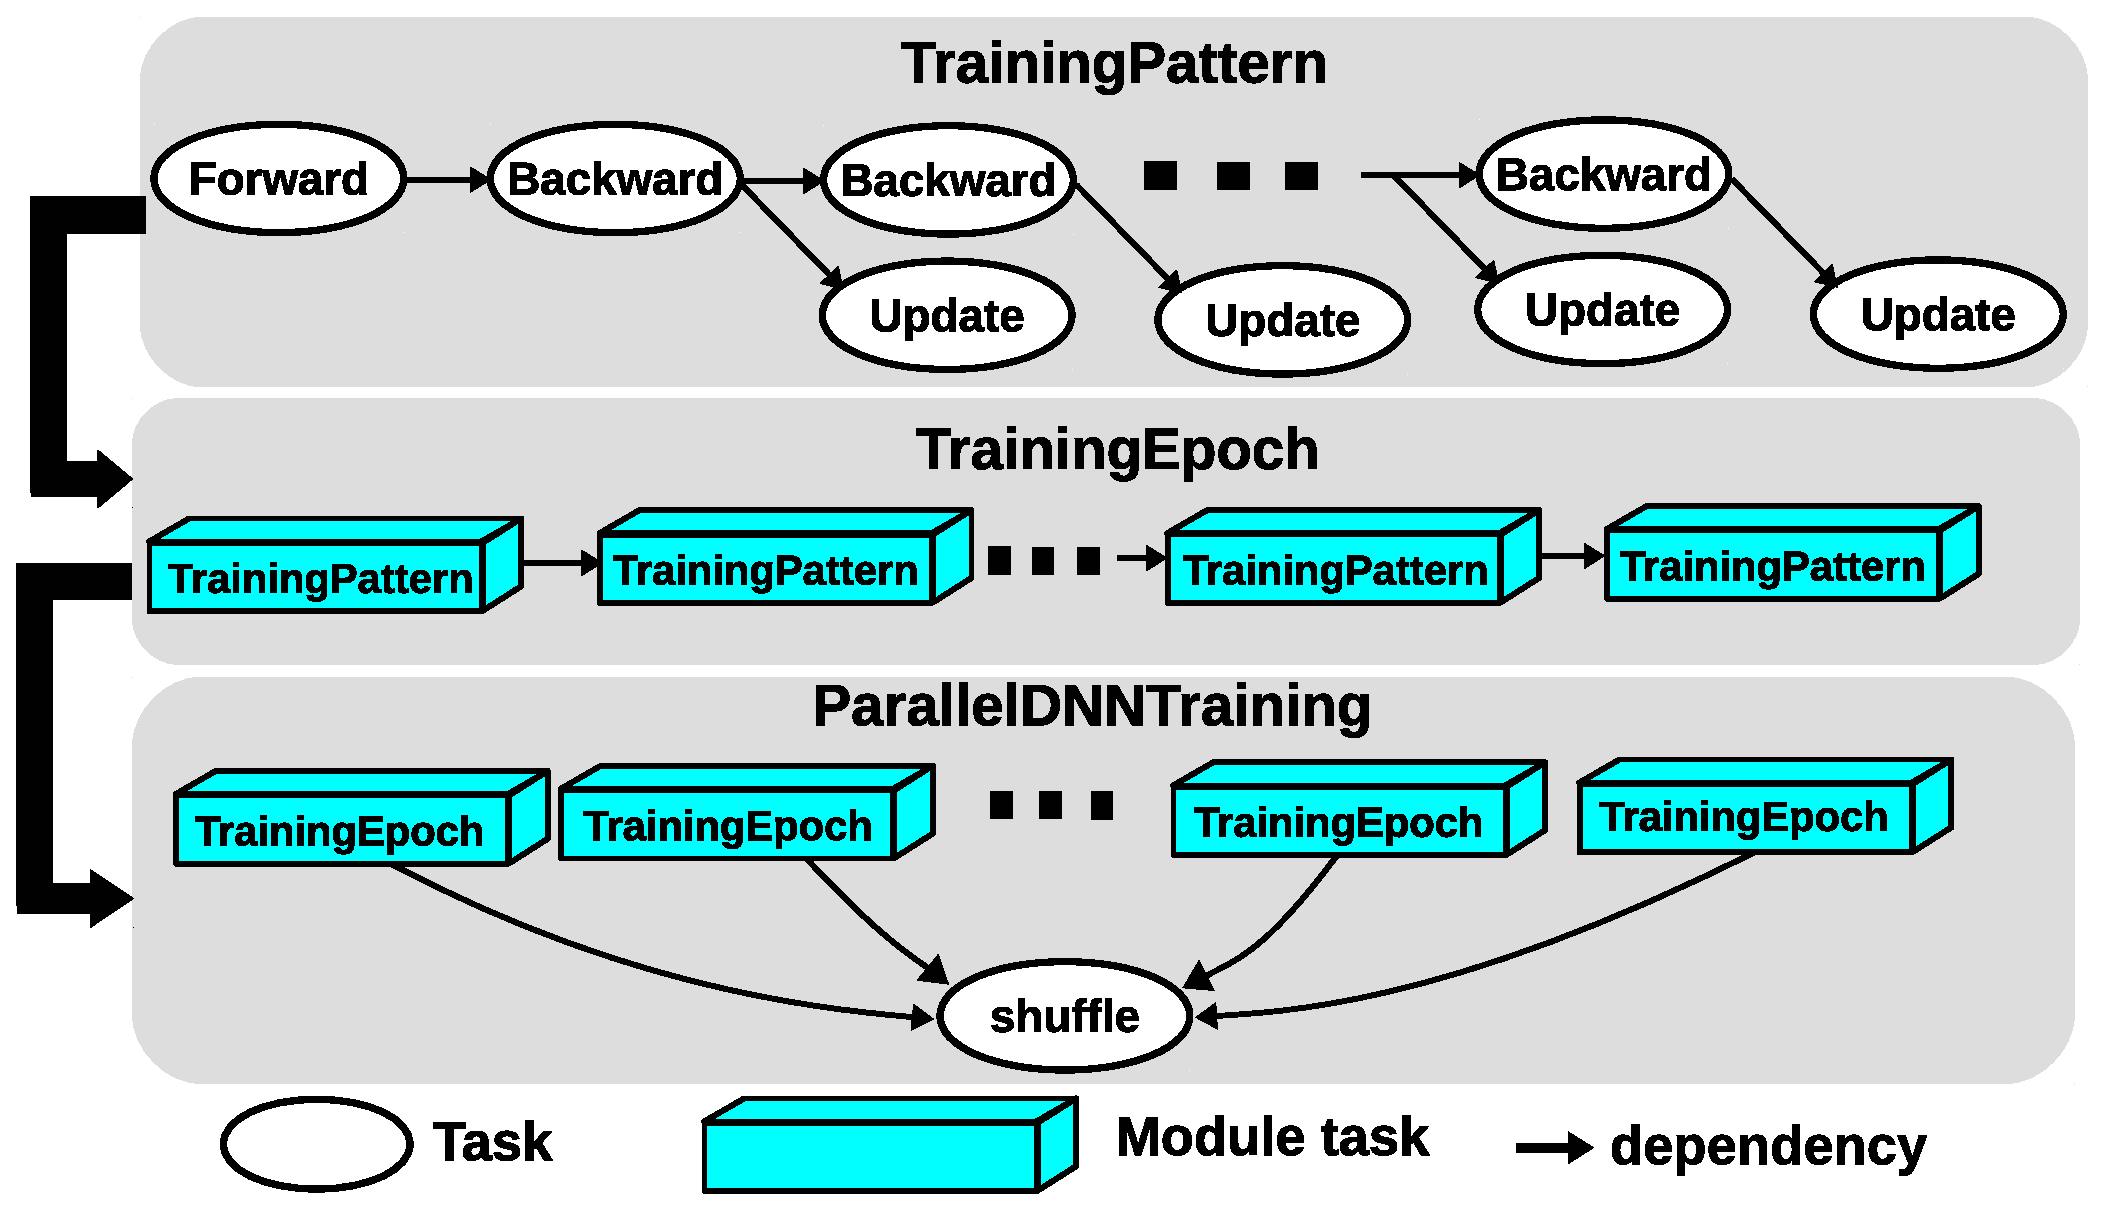
\includegraphics[width=1.\columnwidth]{Fig/parallel_dnn.eps}
  \caption{
    Parallel DNN training through hierarchical composition.
  }
  \label{fig::dnn_composition}
\end{figure}

%  code readability, clarity, maintainability and cleanliness?
% With those framework classes, we can quickly build a DNN training framework for
% each DNN through composing those frameworks. %by simply declaring a \lstinline{ParallelDNNTraining} instance. 
% and huge 
% Unlike a monolithic task dependency graph, %with all tasks mixed, 
% the hierarchical composition is a more organized way to structure 
% The hierarchical composition provides a systematic way to structure 
% the application and can substantially improve the code readability and maintainability.
% The framework composition is very memory-efficient as it stores a pointer to
% the composed task graph rather than flattening it for
% module task execution. 
% Figure~\ref{fig::memory} shows the impact on graph size
% of using composition and non-composition (flat).
% Cpp-Taskflow v2 framework composition uses reference instead of copying the whole task graph, 
%The composability also enables a flexible and efficient 
%debugging process. Since in Cpp-Taskflow v2 a framework is an executable entity, 
%we can examine this parallel DNN training framework from two aspects: 
%vertical inspection, i. e. from a fine-grained level (one iteration) 
%to a coarse-grained level (one epoch) through the bottom-up composition, 
%and horizontal inspection by checking each DNN separately.
% at different levels from the smallest
% unit one iteration to one epoch through the bottom-up design. 
% fine-grained 
% We can also extract and train a specific DNN
% makes the code more well-organized and readable.
% In addition, these DNN frameworks can also
% be reused as building blocks to facilitate the development of other ML applications.

% % This is wavefront experiment data
\begin{figure}[!h]
  \centering

  \pgfplotsset{
    title style={font=\huge},
    label style={font=\normalsize},
    legend style={at={(0.7,0.97)}, anchor=north east}
    %ylabel style={rotate=-90},
  }

  \begin{tikzpicture}[scale=0.5]
    \begin{axis}[
      title=Growth of Tasks (3-layer),
      %bar width=2pt,
      width=\columnwidth,
      %ybar=2pt,
      %symbolic x coords={10,30,50,70,90},
      xtick=data,
      xlabel=Number of iteration,
      ylabel=Number of tasks,
      label style={font=\LARGE},
      x tick label style={font=\Large},
      y tick label style={font=\Large}
    ]
    \addplot table[x=x,y=TF,col sep=space]{Result/memory_usage_3};
    \addplot table[x=x,y=Copy,col sep=space]{Result/memory_usage_3};
    \legend{Composition, Flat}
    \end{axis}
  \end{tikzpicture}
  \begin{tikzpicture}[scale=0.5]
    \begin{axis}[
      title=Growth of Tasks (5-layer),
      %bar width=2pt,
      width=\columnwidth,
      %ybar=2pt,
      %symbolic x coords={10,30,50,70,90},
      xtick=data,
      xlabel=Number of iteration,
      ylabel=Number of tasks,
      label style={font=\LARGE},
      x tick label style={font=\Large},
      y tick label style={font=\Large}
    ]
    \addplot table[x=x,y=TF,col sep=space]{Result/memory_usage_5};
    \addplot table[x=x,y=Copy,col sep=space]{Result/memory_usage_5};
    \legend{Composition, Flat}
    \end{axis}
  \end{tikzpicture}

  \caption{The impact on graph size of using composition and non-composition (flat).}
  \label{fig::memory}
\end{figure}

% The Advantages of Modularization in Programming
%OpenMP only provides tasking directives for annotating the task dependency 
% so we flatten the task 
%so all tasks are deemed to reside in the same graph.
% so we separate the tasks into different functions to 
%we separate the tasks into different functions. 

% We consider the two DNN configurations adopted in~\cite{Huang_19_01}: three
% layers (784x100x30x10) and five layers (784x64x32x16x8x10) with gradient descent
% optimization. 
% The DNN has five layers (784x100x30x10) and we use gradient descent optimization
% For each configuration, we train ten DNNs with randomly selected learning rates in parallel and each batch contains 60 images.  

We train ten DNNs concurrently with each DNN has five layers (784x64x32x16x8x10).
For simplicity, we adopt gradient descent optimization and set the learning rate of each DNN to $0.0001$.
% The DNN has five layers (784x100x30x10) and we use gradient descent optimization for training.
% For simplicity, we set the learning rate to $0.0001$ and 
Table~\ref{table::parallel_dnn_table} is the code complexity analysis reported by Lizard~\cite{lizard}.  
%Cpp-Taskflow v2's implementation is 14\% and 28\% less than the TBB's and OpenMP's
The lines of code (NLOC) of Cpp-Taskflow v2's implementation is 22\% shorter than the TBB's. 
There are two reasons for this: first TBB uses template syntax for task construction and 
second we need to explicitly dispatch the composed graph to execution in TBB's implementation. 
% this is that TBB uses template syntax and 
% This is mainly due to the template syntax and the API design of TBB.
%and Cpp-Taskflow v2 has a lower cyclomatic complexity.
% and 66\% smaller
%than TBB and OpenMP.  
% OpenMP has the longest NLOC due to the enumerating of
% task dependency directives for all DNN configurations.
%The development time is reported by a C++ programmer with 7-year experience on 
%implementing these programs.
%Among those libraries, OpenMP took the longest time to implement as describing
%the irregular dependency with the directive clauses is not very intuitive and 
%is difficult to debug. 
%In contrast, TBB and Taskflow v2 have nearly the same development time as their
%programming models are very similar and 
%xpressing the dependency graph of the
%DNN structure with the graph model is pretty straightforward.
%The development time reflects the impact of programming models on user's productivity 
%even though this might be subjective.
% ease-of-use of different programming models 
% importance of library's programming model. 
\begin{table}[h]
\centering
\caption{Code complexity analysis of the parallel DNN training framework.}
\begin{tabular}{|c|c|c|c|}
\hline
Library & \begin{tabular}[c]{@{}c@{}}NLOC\\  (total)\end{tabular} & \begin{tabular}[c]{@{}c@{}}CCN\\  (avg)\end{tabular} & \begin{tabular}[c]{@{}c@{}}Token\\  (avg)\end{tabular} \\ \hline
Cpp-Taskflow v2 & 60 & 2.0 & 90.6 \\ \hline
TBB & 77 & 2.8 & 125.0 \\ \hline
\end{tabular}
%\caption{Code complexity analysis of the parallel hyperparameter search in three libraries. \\\hspace{\textwidth}NLOC: lines of codes. CCN: cyclomatic complexity number.}
\begin{tablenotes}
\item [1] \hspace{5pt} \textbf{NLOC}: lines of code. \hspace{10pt} \textbf{CCN}: cyclomatic complexity number.
\end{tablenotes}
\label{table::parallel_dnn_table}
\end{table}


%We use 8 cores in this experiment. 
%For each configuration, we train the DNNs in parallel for 10, 30,
%50, 70 and 90 epochs.  For each training we run 10 times and take the average.
% and Figure~\ref{fig::parallel_dnn_layer5} 
We use 10 cores in this experiment and train those DNNs from 10 to 100 epochs.
Figure~\ref{fig::parallel_dnn} plots the two libraries' runtime of the parallel DNN training.
Both libraries exhibit a similar trend in runtime growth when increasing the number of epochs 
and Cpp-Taskflow v2 outperforms TBB in all cases.
%% This is wavefront experiment data
\begin{figure}[!h]
  \centering

  \pgfplotsset{
    title style={font=\huge},
    label style={font=\small},
    legend style={at={(0.7,0.97)}, anchor=north east}
    %ylabel style={rotate=-90},
  }

  \begin{tikzpicture}[scale=0.5]
    \begin{axis}[
      title=3-layer DNN,
      %bar width=2pt,
      width=\columnwidth,
      ybar=2pt,
      symbolic x coords={10,30,50,70,90},
      xtick=data,
      xlabel=Number of epochs,
      ylabel=Runtime (s),
      x tick label style={font=\small},
      y tick label style={font=\small}
    ]
    \addplot table[x=x,y=OMP,col sep=space]{Result/parallel_dnn/layer_3};
    \addplot table[x=x,y=TBB,col sep=space]{Result/parallel_dnn/layer_3};
    \addplot table[x=x,y=TF,col sep=space]{Result/parallel_dnn/layer_3};
    \legend{OpenMP, TBB, Cpp-Taskflow}
    \end{axis}
  \end{tikzpicture}
  \begin{tikzpicture}[scale=0.5]
    \begin{axis}[
      title=5-layer DNN,
      %bar width=2pt,
      width=\columnwidth,
      ybar=2pt,
      symbolic x coords={10,30,50,70,90},
      xtick=data,
      xlabel=Number of epochs,
      ylabel=Runtime (s),
      x tick label style={font=\small},
      y tick label style={font=\small}
    ]
    \addplot table[x=x,y=OMP,col sep=space]{Result/parallel_dnn/layer_5};
    \addplot table[x=x,y=TBB,col sep=space]{Result/parallel_dnn/layer_5};
    \addplot table[x=x,y=TF,col sep=space]{Result/parallel_dnn/layer_5};
    \legend{OpenMP, TBB, Cpp-Taskflow}
    \end{axis}
  \end{tikzpicture}

  \caption{Parallel DNN.}
  \label{fig::parallel_dnn}
\end{figure}

%% This is wavefront experiment data
\begin{figure}[!h]
  \centering

  \pgfplotsset{
    title style={font=\Large},
    label style={font=\small},
    legend style={at={(0.4,0.97)}, anchor=north east}
    %ylabel style={rotate=-90},
  }

  \begin{tikzpicture}[scale=0.9]
    \begin{axis}[
      title=Hyperparamter search of 10 3-layer DNNs,
      enlargelimits,
      compat=newest,
      major grid style=white,
      %nodes near coords,
      enlarge y limits={upper, value=0.1},
      enlarge x limits = 0.2,
      bar width=5pt, 
      enlarge y limits={abs=0.45cm},
      width=\columnwidth,
      ybar=2pt,
      symbolic x coords={0, 10,30,50,70,90,100},
      xtick=data,
      xlabel=Number of epochs,
      ylabel=Runtime (min),
      x tick label style={font=\small},
      y tick label style={font=\small}
    ]
    %\addplot table[x=x,y=OMP,col sep=space]{Result/parallel_dnn/layer_3_mins};
    \addplot table[x=x,y=TBB,col sep=space]{Result/parallel_dnn/layer_3_mins};
    \addplot table[x=x,y=TF,col sep=space]{Result/parallel_dnn/layer_3_mins};
    %\legend{OpenMP, TBB, Cpp-Taskflow}
    \legend{TBB, Cpp-Taskflow}
    \end{axis}
  \end{tikzpicture}

  \caption{Runtime of the parallel 3-layer (784x100x30x10) DNN hyperparameter search.}
  \label{fig::parallel_dnn_layer3}
\end{figure}

%% This is wavefront experiment data
\begin{figure}[!h]
  \centering

  \pgfplotsset{
    title style={font=\Large},
    label style={font=\small},
    legend style={at={(0.4,0.97)}, anchor=north east}
    %ylabel style={rotate=-90},
  }

  \begin{tikzpicture}[scale=0.9]
    \begin{axis}[
      title=Hyperparamter search of 10 5-layer DNNs,
      enlargelimits,
      compat=newest,
      major grid style=white,
      %nodes near coords,
      enlarge y limits={upper, value=0.1},
      enlarge x limits = 0.2,
      bar width=5pt, 
      enlarge y limits={abs=0.45cm},
      width=\columnwidth,
      ybar=2pt,
      symbolic x coords={0, 10,30,50,70,90,100},
      xtick=data,
      xlabel=Number of epochs,
      ylabel=Runtime (min),
      x tick label style={font=\small},
      y tick label style={font=\small}
    ]
    %\addplot table[x=x,y=OMP,col sep=space]{Result/parallel_dnn/layer_5_mins};
    \addplot table[x=x,y=TBB,col sep=space]{Result/parallel_dnn/layer_5_mins};
    \addplot table[x=x,y=TF,col sep=space]{Result/parallel_dnn/layer_5_mins};
    \legend{TBB, Cpp-Taskflow}
    %\legend{OpenMP, TBB, Cpp-Taskflow}
    \end{axis}
  \end{tikzpicture}

  \caption{Runtime of the 5-layer (784x64x32x16x8x10) parallel DNN hyperparameter search.}
  \label{fig::parallel_dnn_layer5}
\end{figure}
 


%% This is wavefront experiment data
\begin{figure}[!h]
  \centering

  \pgfplotsset{
    title style={font=\large},
    label style={font=\small},
    legend style={at={(0.5,0.97)}, anchor=north east}
    %ylabel style={rotate=-90},
  }

  \begin{tikzpicture}[scale=0.95]
    \begin{axis}[
      ylabel near ticks,
      title=Parallel DNN Training (10 CPUs),
      %bar width=2pt,
      width=\columnwidth,
      ybar=2pt,
      symbolic x coords={10,20,30,40,50,60,70,80,90,100},
      xtick=data,
      height=4.7cm,
      width=9.3cm,
      ybar=2pt,
      clip=false,
      separate axis lines,
      bar width=5pt,
      xlabel=Number of epochs,
      ylabel=Runtime (s),
      x tick style={draw=none},
      x tick label style={font=\small},
      y tick label style={font=\small}
    ]
    \addplot table[x=Epoch,y=TBB,col sep=space]{Experiment/total};
    \addplot table[x=Epoch,y=TF,col sep=space]{Experiment/total};
    \legend{TBB, Cpp-Taskflow v2}
    \end{axis}
  \end{tikzpicture}

  \caption{Runtime of training 10 DNNs in parallel.}
  \label{fig::parallel_dnn}
\end{figure}

% This is wavefront experiment data
\begin{figure}[!h]
  \centering

  \pgfplotsset{
    title style={font=\large},
    label style={font=\small},
    legend style={at={(0.5,0.97)}, anchor=north east}
    %ylabel style={rotate=-90},
  }

  \begin{tikzpicture}[scale=0.95]
    \begin{axis}[
      ylabel near ticks,
      %title=Parallel DNN Training (10 CPUs),
      %bar width=2pt,
      width=\columnwidth,
      ybar=2pt,
      symbolic x coords={10,20,30,40,50,60,70,80,90,100},
      xtick=data,
      height=4.7cm,
      width=9.3cm,
      ybar=2pt,
      clip=false,
      separate axis lines,
      bar width=5pt,
      xlabel=Number of epochs,
      ylabel=Runtime (s),
      x tick style={draw=none},
      x tick label style={font=\small},
      y tick label style={font=\small}
    ]
    \addplot table[x=Epoch,y=TBB,col sep=space]{Experiment/camera_total};
    \addplot table[x=Epoch,y=TF,col sep=space]{Experiment/camera_total};
    \legend{TBB, Cpp-Taskflow v2}
    \end{axis}
  \end{tikzpicture}

  \caption{Runtime of training 10 DNNs using 10 cores in parallel.}
  \label{fig::parallel_dnn}
\end{figure}



  %% This is wavefront experiment data
\begin{figure}[!h]
  \centering

  \pgfplotsset{
    title style={font=\large},
    label style={font=\small},
    legend style={at={(0.5,0.97)}, anchor=north east}
    %ylabel style={rotate=-90},
  }

  \begin{tikzpicture}[scale=0.95]
    \begin{axis}[
      ylabel near ticks,
      title=Parallel DNN Training (20 epochs),
      %bar width=2pt,
      width=\columnwidth,
      ybar=2pt,
      symbolic x coords={2,4,6,8,10},
      xtick=data,
      height=4.7cm,
      width=9.3cm,
      ybar=2pt,
      clip=false,
      separate axis lines,
      bar width=5pt,
      xlabel=Number of epochs,
      ylabel=Runtime (s),
      x tick style={draw=none},
      x tick label style={font=\small},
      y tick label style={font=\small}
    ]
    \addplot table[x=CPU,y=TBB,col sep=space]{Experiment/total_scale};
    \addplot table[x=CPU,y=TF,col sep=space]{Experiment/total_scale};
    \legend{TBB, Cpp-Taskflow v2}
    \end{axis}
  \end{tikzpicture}

  \caption{Runtime of training 10 DNNs in parallel.}
  \label{fig::parallel_dnn_cpu}
\end{figure}

%% This is wavefront experiment data
\begin{figure}[!h]
  \centering

  \pgfplotsset{
    title style={font=\LARGE \bfseries},
    label style={font=\huge},
    legend style={at={(0.5,0.97)}, anchor=north east},
    %ylabel style={rotate=-90},
  }

  \begin{tikzpicture}[scale=0.485]
    \begin{axis}[
      title=Hyperparamter search of 3-layer DNNs,
      enlargelimits,
      compat=newest,
      major grid style=white,
      %nodes near coords,
      %enlarge y limits={upper, value=0.1},
      %enlarge x limits = 0.2,
      bar width=13pt, 
      enlarge y limits={abs=0.45cm},
      width=\columnwidth,
      ybar=2pt,
      symbolic x coords={0, 10,30,50,70,90,100},
      xtick=data,
      xlabel=Number of epochs,
      ylabel=Runtime (min),
      label style={font=\LARGE},
      x tick label style={font=\Large},
      y tick label style={font=\Large}
    ]
    %\addplot table[x=x,y=OMP,col sep=space]{Result/parallel_dnn/layer_3_mins};
    \addplot table[x=x,y=TBB,col sep=space]{Result/parallel_dnn/layer_3_mins};
    \addplot table[x=x,y=TF,col sep=space]{Result/parallel_dnn/layer_3_mins};
    %\legend{OpenMP, TBB, Cpp-Taskflow}
    \legend{TBB, Cpp-Taskflow v2}
    \end{axis}
  \end{tikzpicture}
  \begin{tikzpicture}[scale=0.485]
    \begin{axis}[
      title=Hyperparamter search of 5-layer DNNs,
      enlargelimits,
      compat=newest,
      major grid style=white,
      %nodes near coords,
      %enlarge y limits={upper, value=0.1},
      %enlarge x limits = 0.2,
      bar width=13pt, 
      enlarge y limits={abs=0.45cm},
      width=\columnwidth,
      ybar=2pt,
      symbolic x coords={0, 10,30,50,70,90,100},
      xtick=data,
      xlabel=Number of epochs,
      ylabel=Runtime (min),
      label style={font=\LARGE},
      x tick label style={font=\Large},
      y tick label style={font=\Large}
    ]
    %\addplot table[x=x,y=OMP,col sep=space]{Result/parallel_dnn/layer_5_mins};
    \addplot table[x=x,y=TBB,col sep=space]{Result/parallel_dnn/layer_5_mins};
    \addplot table[x=x,y=TF,col sep=space]{Result/parallel_dnn/layer_5_mins};
    \legend{TBB, Cpp-Taskflow v2}
    %\legend{OpenMP, TBB, Cpp-Taskflow}
    \end{axis}
  \end{tikzpicture}
  \caption{Runtime of the parallel hyperparameter search of 3-layer (784x100x30x10) and 5-layer (784x64x32x16x8x10) DNNs.}
  \label{fig::parallel_dnn_layers}
\end{figure}

%For 90 epochs, the performance margin between TBB and Cpp-Taskflow v2 is 9\% and 6\% 
%for the 3-layer and 5-layer DNNs respectively. 
% and then are the TBB and Taskflow.  
%The performance difference between Cpp-Taskflow v2 and TBB is due to 
%the overhead of the task graph composition.  Composition allocates
%additional memory for the module tasks, and a module task execution requires 
%more work than a regular task execution in order to deploy the composed framework.  


\subsection{VLSI Timing Analysis}
%We demonstrate using Cpp-Taskflow v2 to emulate VLSI timing analysis. 
%implement a real-world application, VLSI timing analysis. 
The second application is VLSI timing analysis. 
Timing analysis is an important step in 
circuit design as a circuit must meet the timing requirements before 
tape-out~\cite{Huang_16_01}~\cite{Huang_15_01}.  
Timing analysis contains different workloads such as timing simulation and correlation,
and each workload can be managed either by a tool or a library. % which is developed and maintained by a team.
In order to run a complete timing analysis, users have to integrate libraries into their  
programs and write hard-coded scripts to compose those tools.  Obviously,
hard-coded script is not flexible and is very difficult to scale up to complex control flow.  
% With Cpp-Taskflow v2, we can use the framework interface to quickly compose those tools 
% together to emulate the timing analysis flow. 
In this experiment, we demonstrate using Cpp-Taskflow v2 to quickly compose those tools 
together to emulate the timing analysis flow. 
The idea is to encapsulate each tool in a task 
and those tasks use process fork to execute the tools. 
% This method can effectively handle the complex control flow 
Our method can shorten the analysis runtime by letting tools run concurrently and 
can also effectively handle the complex control flow.   

%Figure~\ref{fig::vlsi_timing} depicts the frameworks in the proposed parallel timing analysis flow.
Figure~\ref{fig::vlsi_timing} depicts the timing analysis flow.
%each framework is a C++ 
%each framework corresponds to a task dependency graph.
In the process framework, we launch multiple timers
with each running the timing analysis for a scenario\footnote{In this experiment, a scenario 
denotes a different design constraint.} 
and dumping the top 100 critical paths to disk. After timers finish, 
those paths are read into memory by a reader task. 
A simulation framework composes multiple process frameworks to parallelize the
path reading. To find the correlation between each pair of scenarios using
those critical paths, we create a scenario task to calculate the correlation
coefficients between a scenario and others. Those scenario tasks are
gathered into the scenario framework.  Lastly, we build a timing analysis
framework by composing the simulation framework and the scenario framework. 

\begin{figure}[!h]
  \centering
  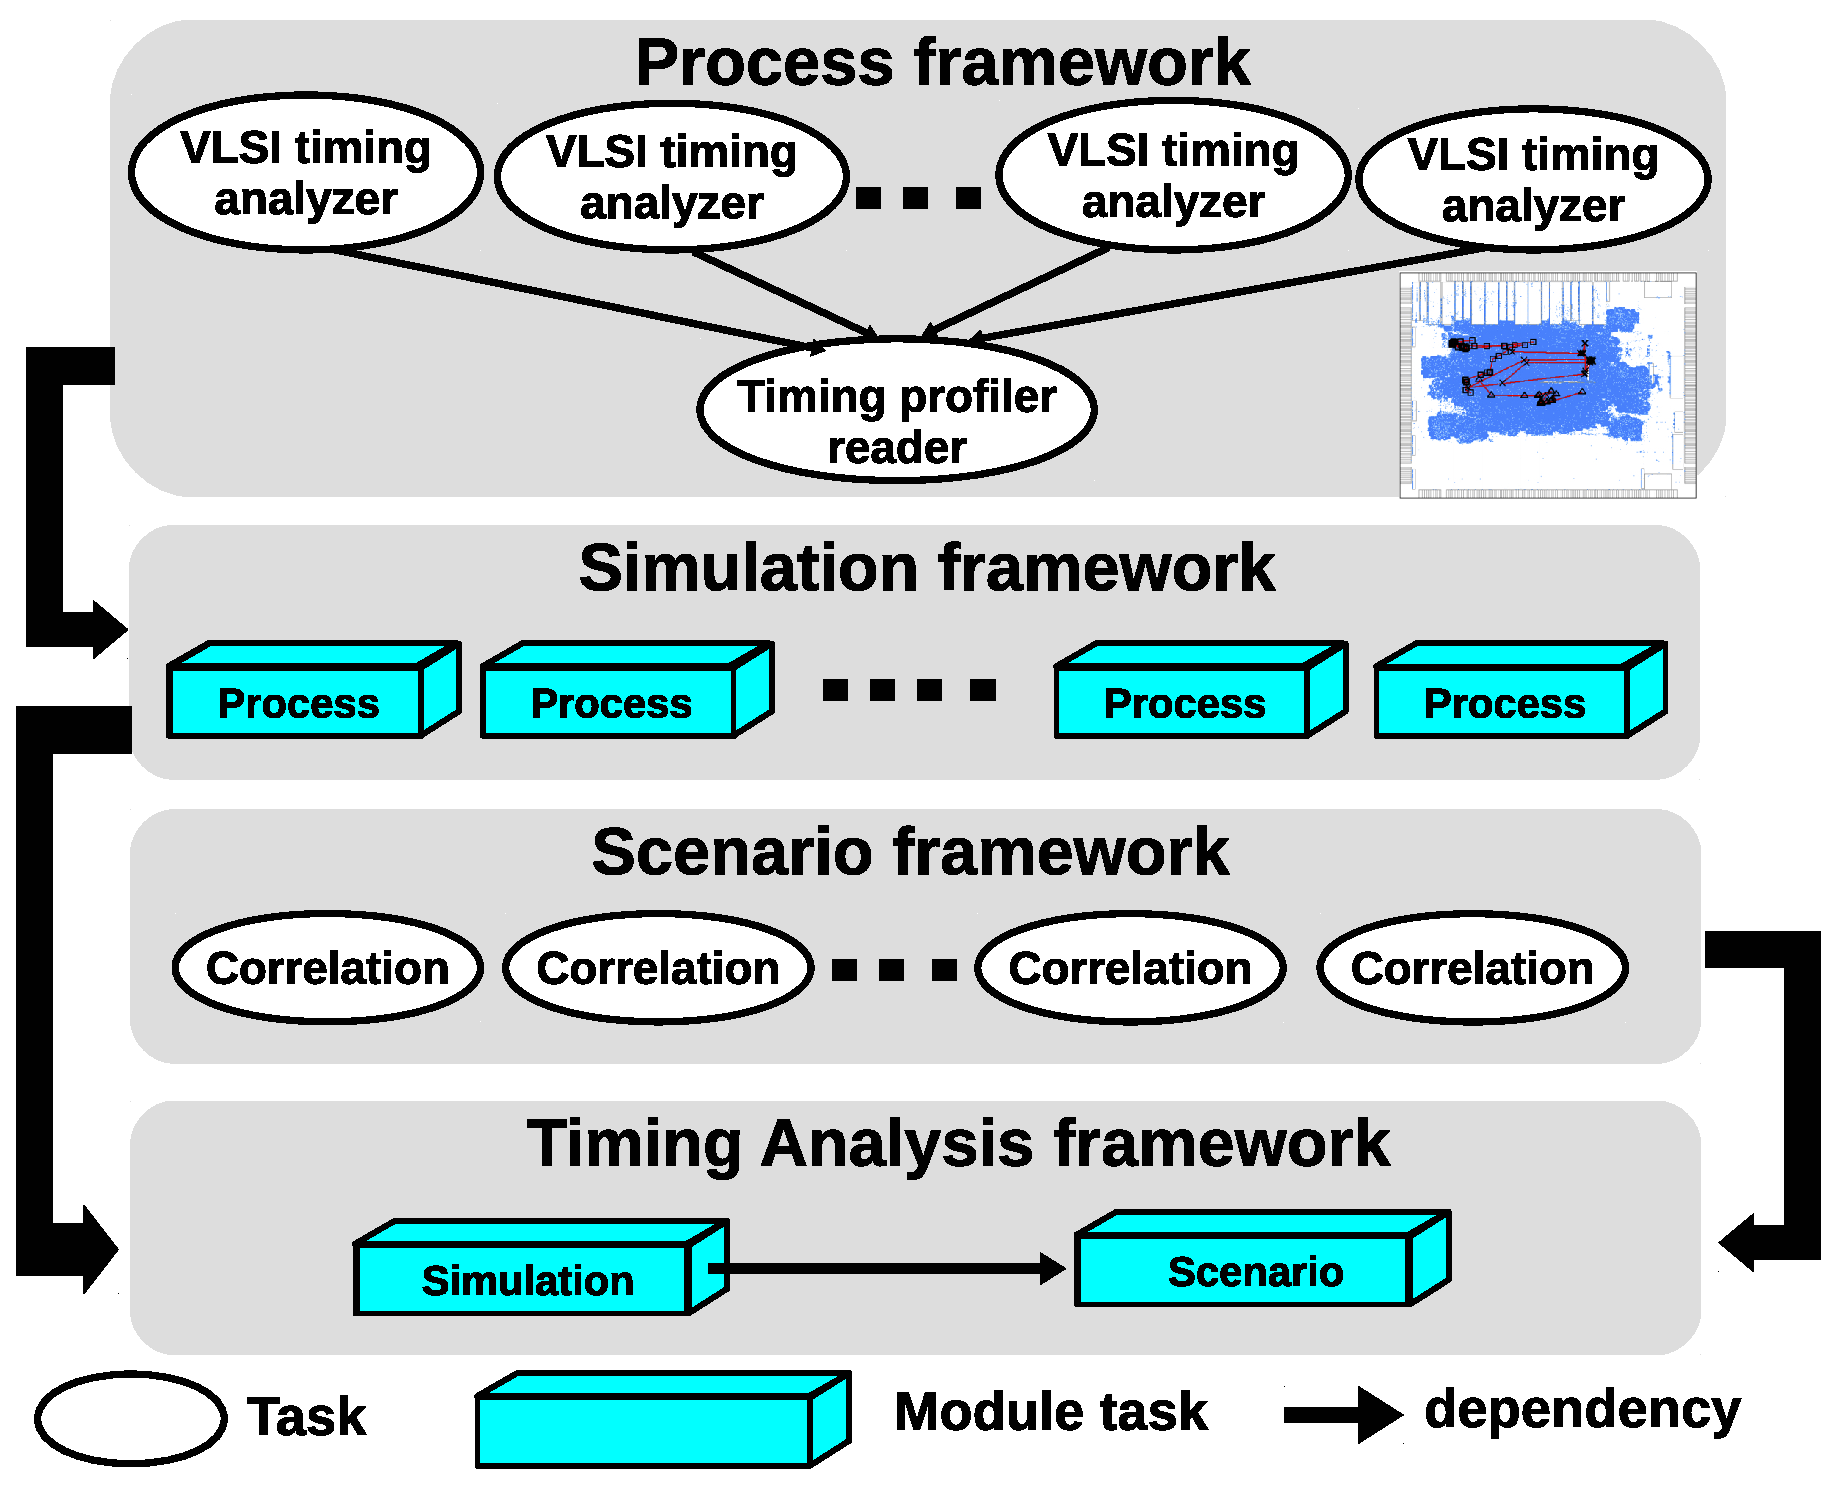
\includegraphics[width=.9\columnwidth]{Fig/vlsi_timing.eps}
  \caption{
    A parallel VLSI timing analysis framework.
  }
  \label{fig::vlsi_timing}
\end{figure}

%As OpenMP has no task graph construct, we compare the flow implementations of Cpp-Taskflow v2 and TBB.
%we create individual C++ struct for the process framework, simulation framework, and scenario framework, 
We create individual C++ struct for the first three frameworks by inheriting \lstinline{tf::Taskflow}
and build the timing analysis framework in a single function (top) using these frameworks. 
We use OpenTimer~\cite{Huang_15_01}, an
% frameworks in a top function. We use OpenTimer~\cite{Huang_15_01}, an
open-source VLSI timing analyzer, to perform static timing analysis (STA). 
Table~\ref{table::vlsi_timing_table} shows the code complexity of each
implementation measured by Lizard.  The results show that Cpp-Taskflow v2 takes 
fewer lines of code than TBB.
%same cyclomatic complexity as TBB but with 32\% less NLOC in total. %and 19\% tokens in total. 
% Table~\ref{table::vlsi_timing_table} shows the code complexity of each
% framework class and the top function measured by Lizard.  Cpp-Taskflow v2 has the
% same cyclomatic complexity as TBB but with 32\% less NLOC in total. %and 19\% tokens in total. 

\begin{table}[]
  \centering 
  \caption{Code complexity analysis of the timing analysis flow. The first table is the whole file and the second table is for 
  individual framework.}
  \begin{tabular}{|c|c|c|c|}
    \hline
  Library & \begin{tabular}[c]{@{}c@{}}NLOC (total)\end{tabular} & \begin{tabular}[c]{@{}c@{}}CCN (avg)\end{tabular} & \begin{tabular}[c]{@{}c@{}}Token (avg)\end{tabular} \\ \hline
    Cpp-Taskflow v2 & 61 & 3.0 & 132 \\ \hline
    TBB & 104 & 2.6 & 106.6 \\ \hline
  \end{tabular}
\newline
\vspace*{0.2 cm}
\newline
  \begin{tabular}{|c|c|c|c|c|c|c|}
    \hline
    \multirow{2}{*}{Framework} & \multicolumn{2}{c|}{NLOC (total)} & \multicolumn{2}{c|}{CCN (avg)} & \multicolumn{2}{c|}{Token (avg)} \\ \cline{2-7} 
     & TF & TBB & TF & TBB & TF & TBB \\ \hline
    Process & 10 & 14 & 2 & 2 & 118 & 155 \\ \hline
    Simulation & 5 & 9 & 2 & 2 & 47 & 63 \\ \hline
    Scenario & 15 & 16 & 4 & 4 & 137 & 155 \\ \hline
    Top & 23 & 29 & 4 & 4 & 226 & 283 \\ \hline
  \end{tabular}
  \begin{tablenotes}
  \item [1] \hspace{5pt} \textbf{NLOC}: lines of code. \hspace{10pt} \textbf{CCN}: cyclomatic complexity number.
  \end{tablenotes}
  \label{table::vlsi_timing_table}
\end{table}


% \begin{table}[h]
% \caption{Code complexity analysis of the VLSI timing analysis flow using TBB and Cpp-Taskflow v2.}
% \centering
% \begin{tabular}{|c|c|c|c|c|}
% \hline
% \multicolumn{2}{|c|}{Code complexity} & NLOC & CCN & Token \\ \hline
% \multirow{2}{*}{\begin{tabular}[c]{@{}c@{}}Process\\ Framework\end{tabular}} & TBB & 20 & 2 & 155 \\ \cline{2-5} 
%  & Cpp-Taskflow v2 & 10 & 2 & 118 \\ \hline
% \multirow{2}{*}{\begin{tabular}[c]{@{}c@{}}Simulation\\ Framework\end{tabular}} & TBB & 11 & 2 & 63 \\ \cline{2-5} 
%  & Cpp-Taskflow v2 & 5 & 2 & 47 \\ \hline
% \multirow{2}{*}{\begin{tabular}[c]{@{}c@{}}Scenario\\ Framework\end{tabular}} & TBB & 16 & 4 & 155 \\ \cline{2-5} 
%  & Cpp-Taskflow v2 & 15 & 4 & 137 \\ \hline
% \multirow{2}{*}{\begin{tabular}[c]{@{}c@{}}Top\\ function\end{tabular}} & TBB & 31 & 4 & 283 \\ \cline{2-5} 
%  & Cpp-Taskflow v2 & 23 & 4 & 228 \\ \hline
% \end{tabular}
% \begin{tablenotes}
% \item [1] \hspace{7pt} \textbf{NLOC}: lines of codes. \hspace{10pt} \textbf{CCN}: cyclomatic complexity number.
% \end{tablenotes}
% \label{table::vlsi_timing_table}
% \end{table} 

Next for performance profiling, we create 1024 design constraints with each representing a scenario.
%for each % to generate 1024 scenarios
% scenario 
For each scenario we launch a timer % with the 45nm NanGate cell library~\cite{tau_2015} 
to analyze the industrial circuit tv80 (5.3k gates and 5.3k nets)~\cite{tau_2015} and 
group 8 timers in a process framework.
% we launch 1024 timers to analyze the industrial
% circuit tv80 (5.3k gates and 5.3k nets) with 45nm NanGate cell
% library~\cite{tau_2015} under 1024 timing constraints. 
Figure~\ref{fig::tv80} shows the results of scaling from 1 core to 14 cores.
Both TBB's and Cpp-Taskflow v2's runtimes exhibit the same scaling and
are very close in all cases.
%% This is wavefront experiment data
\begin{figure}[!h]
  \centering

  \pgfplotsset{
    title style={font=\Large},
    label style={font=\small},
    %legend style={at={(0.35,0.97)}, anchor=north east} 
    legend style={at={(0.7,0.97)}, anchor=north east}
    %ylabel style={rotate=-90},
  }

  \begin{tikzpicture}[scale=0.9]
    % Fix: CPU=14, Repeat=100
    \begin{axis}[
      title=VSLI Timing Analysis,
      bar width=3pt,
      width=\columnwidth,
      ybar=2pt,
      symbolic x coords={1,2,3,4,5,6,7,8,9,10,11,12,13,14},
      xtick=data,
      xlabel=Number of CPUs,
      ylabel=Runtime (s),
      x tick label style={font=\small},
      y tick label style={font=\small}
    ]
    \addplot table[x=x,y=TBB,col sep=space]{Result/timing_analysis/tv80.csv};
    \addplot table[x=x,y=TF,col sep=space]{Result/timing_analysis/tv80.csv};
    \legend{TBB, Cpp-Taskflow v2}
    \end{axis}
  \end{tikzpicture}

  \caption{Runtime comparisons of the proposed VLSI timing analysis flow on circuit tv80 using TBB and Cpp-Taskflow v2}
  \label{fig::tv80}
\end{figure}

%% This is wavefront experiment data
\begin{figure}[!h]
  \centering

  \pgfplotsset{
    title style={font=\large},
    label style={font=\small},
    %legend style={at={(0.35,0.97)}, anchor=north east} 
    legend style={at={(0.9,0.9)}, anchor=north east}
    %ylabel style={rotate=-90},
  }

  \begin{tikzpicture}[scale=0.9]
    % Fix: CPU=14, Repeat=100
    \begin{axis}[
      ylabel near ticks,
      title=VSLI Timing Analysis,
      bar width=3pt,
      width=\columnwidth,
      ybar=2pt,
      %xtick distance=2,
      symbolic x coords={1,2,3,4,5,6,7,8,9,10,11,12,13,14},
      xtick=data,
      bar width=4pt,
      clip=false,
      separate axis lines,
      xlabel=Number of CPUs,
      ylabel=Runtime (s),
      height=5.0cm,
      width=9.4cm,
      x tick style={draw=none},
      %y tick style={draw=none},
      x tick label style={font=\small},
      y tick label style={font=\small}
    ]
    \addplot table[x=Thread,y=TBB,col sep=space]{Experiment/timer_all};
    \addplot table[x=Thread,y=TF,col sep=space]{Experiment/timer_all};
    \legend{TBB, Cpp-Taskflow v2}
    \end{axis}
  \end{tikzpicture}

  \caption{Runtime comparisons of the proposed VLSI timing analysis flow on circuit tv80 using TBB and Cpp-Taskflow v2}
  \label{fig::tv80}
\end{figure}

% This is wavefront experiment data
\begin{figure}[!h]
  \centering

  \pgfplotsset{
    title style={font=\large},
    label style={font=\small},
    %legend style={at={(0.35,0.97)}, anchor=north east} 
    legend style={at={(0.9,0.9)}, anchor=north east}
    %ylabel style={rotate=-90},
  }

  \begin{tikzpicture}[scale=0.9]
    % Fix: CPU=14, Repeat=100
    \begin{axis}[
      ylabel near ticks,
      %title=VSLI Timing Analysis,
      bar width=3pt,
      width=\columnwidth,
      ybar=2pt,
      %xtick distance=2,
      symbolic x coords={1,2,3,4,5,6,7,8,9,10,11,12,13,14},
      xtick=data,
      bar width=4pt,
      clip=false,
      separate axis lines,
      xlabel=Number of cores,
      ylabel=Runtime (s),
      height=5.0cm,
      width=9.4cm,
      x tick style={draw=none},
      %y tick style={draw=none},
      x tick label style={font=\small},
      y tick label style={font=\small}
    ]
    \addplot table[x=Thread,y=TBB,col sep=space]{Experiment/camera_timer_all};
    \addplot table[x=Thread,y=TF,col sep=space]{Experiment/camera_timer_all};
    \legend{TBB, Cpp-Taskflow v2}
    \end{axis}
  \end{tikzpicture}

  \caption{Runtime comparisons of the proposed VLSI timing analysis flow on circuit tv80 using TBB and Cpp-Taskflow v2}
  \label{fig::tv80}
\end{figure}


% \section{Related Work} 
% Existing parallel programming libraries have enabled task parallelism in various ways. 
% Intel Threading Building Blocks (TBB) is a C++ parallel programming library that
% supports generic parallel patterns like DOALL and DOPIPE parallelism,
% concurrent data structures and task-based parallelism~\cite{tbb}. 
% %For task-based parallelism, TBB lets users formulate the tasks with their dependency as 
% %a data flow graph where nodes are tasks and edges denote the data flow.
% %TBB also provides several types of nodes to support different data communication methods between tasks.
% For task-based parallelism, TBB lets users formulate the tasks with their dependency as 
% a data flow graph.
% %This is similar to Cpp-Taskflow v2 task dependency graph.
% The flow graph can be repeatedly executed but TBB does not provide any API for
% direct flow graph composition.  To emulate graph composition, a viable way is
% to explicitly capture a flow graph into a task of another flow graph. A significant
% drawback of this method is users have to manually dispatch the captured flow
% graph to execution, which is quite inconvenient and leads to longer lines of
% code. 
% 
% % bury bug? 
% % Doing this is not as convenient as
% % Cpp-Taskflow v2 as users have to manually dispatch the captured flow graph
% % Cpp-Taskflow's task dependency graph is similar to TBB's flow graph. 
% %However, writing parallel code using TBB is very verbose due to the 
% %heavy use of template in TBB. Template decreases the code readability and 
% %increases the development effort as debugging templated code could be onerous.
% 
% OpenMP~\cite{openmp} includes task-based parallelism by providing task directives starting from OpenMP 3.0.
% Through those task directives users can spawn tasks and specify the task dependency via the 
% task depend clause. 
% % This directive-based programming scheme has several issues.
% % First, it relies on the compiler support.
% % Second, code with the compiler directives is not readable and difficult to debug
% % when encountering complex task dependency. 
% % Third, users must organize the dependent tasks in a specific order to ensure the  
% % task execution is correct under a single thread.
% %However, the task in OpenMP is not a real object and OpenMP has no concept of a single
% However, OpenMP has no directive for creating a single task dependency graph. In
% other words, in OpenMP the whole application can be seen as a
% monolithic task graph and it is unable to do task dependency graph
% composition like Cpp-Taskflow v2 in OpenMP.
% % and there is no 
% % graph composition 
% % In addition, OpenMP is not object-oriented. 
% Similarly, OmpSs is a programming model built on top of OpenMP to 
% enable asynchronous parallelism~\cite{ompss}. As it adopts the directive-based
% approach as OpenMP for tasking, it also suffers from the aforementioned issues of OpenMP.
% Intel Cilk Plus~\cite{cilk_plus} extends the C and C++ programming language to enable
% task parallelism, but it does not have task dependency annotation nor task graph. 
% 
% Aside from the programming libraries, there are programming languages and
% runtime systems designed with task-based parallelism to be employed for cluster
% computing. %For example, 
% Charm++~\cite{charmplusplus} provides a programming language together with a runtime system
% to allow users write parallel programs that to scale from a single machine to 
% a cluster. Charm++ has also introduced composability ~\cite{charm_compose} to improve performance.  
% The composability of Charms++ is to interleave operations between parallel
% modules during runtime, which is different from the task graph
% composition in Cpp-Taskflow v2.
% Chapel~\cite{chapel} and
% X10~\cite{X10_paper}~\cite{X10} are programming languages based on the
% partitioned global address space (PGAS) programming model. 
% HPX~\cite{HPX} is a runtime system based on the PGAS programming model for developing 
% parallel and distributed C++ programs.
% Legion~\cite{Legion} introduces a programming model that considers the data locality 
% to achieve high performance computing in heterogeneous environment.
% In conclusion, those libraries have offered task parallelism but they do not have the
% same task graph composition capability as Cpp-Taskflow v2. 





\section{Conclusions}
This paper presents Cpp-Taskflow v2, a parallel programming library on 
composable task graph.  Cpp-Taskflow v2 introduces a task graph composition
interface to enable composable parallel programming. 
Users can use the composition interface to quickly build a large parallel 
program through composing modular and reusable task graphs.
The experimental results show that Cpp-Taskflow v2 can achieve comparable
performance to Intel Threading Building Blocks with fewer lines of code.
Future work will focus on extension to heterogeneous computing,
especially under the mixed workload of CPUs and GPUs.
%Cpp-Taskflow v2 not only has concise and
%intuitive tasking APIs, but also provides a flexible framework interface to let
%users take the advantage of its composability, modularity and reusability to
%quickly build complex parallel applications.  
% We have compared Cpp-Taskflow v2 
% with Intel Threading Building Blocks using real-world applications. The results show Cpp-Taskflow v2's outperforms 
% TBB on the task scheduling and the task graph composition can effectively reduce the code complexity 
% of a machine learning hyperparameter search application and a VLSI timing analysis application.

\section{Acknowledgement}
This work is supported by NSF Grant CCF-1718883 and DARPA Grant FA 8650-18-2-7843.



\bibliographystyle{unsrt}
\bibliography{hpec}    

%IEEE conference templates contain guidance text for composing and formatting conference papers. Please ensure that all template text is removed from your conference paper prior to submission to the conference. Failure to remove the template text from your paper may result in your paper not being published.

\end{document}
